\documentclass[oneside,numbers,spanish]{ezthesis}
\usepackage[utf8]{inputenc}
\usepackage{tcolorbox}
\usepackage{listings}
\usepackage{graphicx}
\usepackage{pdfpages}
\usepackage{lscape}
\usepackage{xcolor}
\usepackage{todonotes}
\usepackage{lipsum}
\usepackage{bbding}
\usepackage{pifont}
\usepackage{wasysym}
\usepackage{amssymb}
\usepackage{natbib}
\usepackage{bm}
\usepackage{color}    
\usepackage{enumitem}
\definecolor{blue}{rgb}{1,0.5,0}

%Para hacer comentarios

\makeatletter
\def\myaddcontentsline#1#2#3{%
  \addtocontents{#1}{\protect\contentsline{#2}{#3}{see \thesection\ at p. \thepage}{}}}
\renewcommand{\@todonotes@addElementToListOfTodos}{%
    \if@todonotes@colorinlistoftodos%
        \myaddcontentsline{tdo}{todo}{{%
            \colorbox{\@todonotes@currentbackgroundcolor}%
                {\textcolor{\@todonotes@currentbackgroundcolor}{o}}%
            \ \@todonotes@caption}}%
    \else%
        \myaddcontentsline{tdo}{todo}{{\@todonotes@caption}}%
    \fi}%
\newcommand*\mylistoftodos{%
  \begingroup
       \setbox\@tempboxa\hbox{see 9.9 at p. 99}%
       \renewcommand*\@tocrmarg{\the\wd\@tempboxa}%
       \renewcommand*\@pnumwidth{\the\wd\@tempboxa}%
       \listoftodos%
  \endgroup
}
\makeatother






\lstset{
basicstyle=\ttfamily,
keywordstyle=\bfseries,
showstringspaces=false,
columns = fullflexible,
mathescape = true,
language=R,
%%frame = single,  
framexleftmargin=15pt}



%% # Opciones disponibles para el documento #
%%
%% Las opciones con un (*) son las opciones predeterminadas.
%%
%% Modo de compilar:
%%   draft            - borrador con marcas de fecha y sin im'agenes
%%   draftmarks       - borrador con marcas de fecha y con im'agenes
%%   final (*)        - version final de la tesis
%%
%% Tama'no de papel:
%%   letterpaper (*)  - tama'no carta (Am'erica)
%%   a4paper          - tama'no A4    (Europa)
%%
%% Formato de impresi'on:
%%   oneside          - hojas impresas por un solo lado
%%   twoside (*)      - hijas impresas por ambos lados
%%
%% Tama'no de letra:
%%   10pt, 11pt, o 12pt (*)
%%
%% Espaciado entre renglones:
%%   singlespace      - espacio sencillo
%%   onehalfspace (*) - espacio de 1.5
%%   doublespace      - a doble espacio
%%
%% Formato de las referencias bibliogr'aficas:
%%   numbers          - numeradas, p.e. [1]
%%   authoryear (*)   - por autor y a'no, p.e. (Newton, 1997)
%%
%% Opciones adicionales:
%%   spanish         - tesis escrita en espa'nol
%%
%% Desactivar opciones especiales:
%%   nobibtoc   - no incluir la bibiolgraf'ia en el 'Indice general
%%   nofancyhdr - no incluir "fancyhdr" para producir los encabezados
%%   nocolors   - no incluir "xcolor" para producir ligas con colores
%%   nographicx - no incluir "graphicx" para insertar gr'aficos
%%   nonatbib   - no incluir "natbib" para administrar la bibliograf'ia

%% Paquetes adicionales requeridos se pueden agregar tambi'en aqu'i.
%% Por ejemplo:
%\usepackage{subfig}
%\usepackage{multirow}

%% # Datos del documento #
%% Nota que los acentos se deben escribir: \'a, \'e, \'i, etc.
%% La letra n con tilde es: \~n.

\author{JULIA ANGELINI}
\title{Paquete de R y aplicación Web para el análisis de datos provenientes de ensayos multiambientales}
\degree{TRABAJO FINAL PARA OPTAR AL TITULO DE ESPECIALISTA EN BIOINFORMÁTICA}
\supervisor{DIRECTOR: Gerardo Cervigni \\
			CO-DIRECTOR: Marcos Prunello}
\institution{UNIVERSIDAD NACIONAL DE ROSARIO}
\faculty{FACULTAD DE CIENCIAS AGRARIAS}
\submitdate{AÑO: 2019}
%% # M'argenes del documento #
%% 
%% Quitar el comentario en la siguiente linea para austar los m'argenes del
%% documento. Leer la documentaci'on de "geometry" para m'as informaci'on.

\geometry{top=30mm,bottom=30mm,inner=30mm,outer=20mm}

 
%% El siguiente comando agrega ligas activas en el documento para las
%% referencias cruzadas y citas bibliogr'aficas. Tiene que ser *la 'ultima*
%% instrucci'on antes de \begin{document}.
\hyperlinking
\begin{document}

%% En esta secci'on se describe la estructura del documento de la tesis.
%% Consulta los reglamentos de tu universidad para determinar el orden
%% y la cantidad de secciones que debes de incluir.

%% # Portada de la tesis #
%% Mirar el archivo "titlepage.tex" para los detalles.
\begin{titlepage}
  \TitleBlock{
  \centering 
\includegraphics[height=3cm, keepaspectratio=true]{./Graficos/UNR.png}
  
  \vspace*{0.15cm}
  \normalsize \scshape \textbf{\insertfaculty} \\
  \vspace*{0.15cm}
  \textbf{\insertinstitution}
	}
  \TitleBlock[\vspace*{1.5cm}]{\large\scshape \textbf{\inserttitle}}
  \vspace*{0.55cm}

  \TitleBlock[\vspace*{1.5cm}]{\normalsize \scshape \textbf{\insertauthor}}
  \TitleBlock[\vspace*{0.75cm}]{\normalsize \scshape \textbf{\insertdegree} \\
  \rule{5cm}{0.2mm}}
  \TitleBlock[\vspace*{1.5cm}]{\normalsize \scshape 
  \textbf{\insertsupervisor}}
  \TitleBlock[\vspace*{1.5cm}]{\textbf{\insertsubmitdate}}
\end{titlepage}


%% # Prefacios #
%% Por cada prefacio (p.e. agradecimientos, resumen, etc.) crear
%% un nuevo archivo e incluirlo aqu'i.
%% Para m'as detalles y un ejemplo mirar el archivo "gracias.tex".
%% Las secciones del "prefacio" inician con el comando \prefacesection{T'itulo}
%% Este tipo de secciones *no* van numeradas, pero s'i aparecen en el 'indice.
%%
%% Si quieres agregar una secci'on que no vaya n'umerada y que *tampoco*
%% aparesca en el 'indice, usa entonces el comando \chapter*{T'itulo}
%%
%% Recuerda que aqu'i ya puedes escribir acentos como: 'a, 'e, 'i, etc.
%% La letra n con tilde es: 'n.

%\thispagestyle{empty}
\begin{center}
\textbf{\Large{Paquete de R y aplicación web Shiny para el análisis de datos provenientes de ensayos multiambientales}}
\end{center}

\vspace{1.5cm}

\begin{center}
Julia Angelini

\vspace{0.5cm}
Licenciada en Estadística – Universidad Nacional de Rosario
\end{center}
\vspace{1.5cm}
Este Trabajo Final es presentado como parte de los requisitos para optar al grado académico de Especialista en \textbf{Bioinformática}, de la Universidad Nacional de Rosario y no ha sido previamente presentada para la obtención de otro título en ésta u otra Universidad. El mismo contiene los resultados obtenidos en investigaciones llevadas a cabo en \textbf{el Centro de Estudios Fotosintéticos y Bioquímicos (CEFOBI)}, durante el período comprendido entre \textbf{los años 2017 y 2021}, bajo la dirección del \textbf{Dr. Gerardo Cervigni} y la co-dirección del \textbf{Mgs. Marcos Prunello}.  

\vspace{1.25cm}
Nombre y firma del autor\\
\vspace{0.05cm}
\hspace{0.95cm}Lic. Julia Angelini

\vspace{1.25cm}
Nombre y firma del Director\\
\vspace{0.05cm}
\hspace{0.95cm}Dr. Gerardo Cervigni
 
\vspace{1.25cm}
Nombre y firma del Co - Director\\
\vspace{0.05cm}
\hspace{1.3cm}Mgs. Marcos Prunello
\vspace{1.85cm}

\rightline{Defendida: \rule{3cm}{0.4pt} de 20\rule{1cm}{0.4pt}.}


%% Por si alguien tiene curiosidad, este "simp'atico" agradecimiento est'a
%% tomado de la "Tesis de Lydia Chalmers" basada en el universo del programa
%% de televisi'on Buffy, la Cazadora de Vampiros.
%% http://www.buffy-cazavampiros.com/Spiketesis/tesis.inicio.htm


\pagestyle{plain}
\pagenumbering{roman}
%% Las secciones del "prefacio" inician con el comando \prefacesection{T'itulo}
%% Este tipo de secciones *no* van numeradas, pero s'i aparecen en el 'indice.
%%
%% Si quieres agregar una secci'on que no vaya n'umerada y que *tampoco*
%% aparesca en el 'indice, usa entonces el comando \chapter*{T'itulo}
%%
%% Recuerda que aqu'i ya puedes escribir acentos como: 'a, 'e, 'i, etc.
%% La letra n con tilde es: 'n.

\chapter*{Agradecimientos}
\begin{spacing}{1}

\emph{En este trabajo final, directa o indirectamente, participaron muchas personas a las que les quiero agradecer.}

\emph{En primer lugar al Dr. Gerardo Cervigni por haberme propuesto realizar la Especialización Bioinformática, compartir su conocimiento y experiencia a lo largo de todo el proceso, contagiando su pasión, entusiasmo y energía. }

\emph{Al Mgs. Marcos Prunello por acompañarme en el desarrollo del trabajo final, por su dedicación, sus consejos y su ejemplo que me incentiva a superarme como profesional. Sin su confianza, apoyo y atención, este trabajo no hubiera sido posible. No sólo me enriquecí en lo académico sino también con la amistad que pudimos forjar. }

\emph{Al Centro Computacional del Centro Científico Teconológico de Rosario, miembro del Sistema Nacional de Computación de Alto Rendimiento, por la predisposición, asesoramiento e instalación de los recursos adicionales necesarios para este trabajo. }

\emph{Al Dr. Sergio Arciniegas Alarcón por su predisposición en la inclusión de los avances metodológicos realizados por su equipo de investigación en este trabajo.}

\emph{A mis compañeros de la Especialización, por las largas horas de cursos, mates y almuerzos. En especial, a Jor y Lu, por el aliento en todo momento, por compartir excelentes momentos y porque gracias a la ayuda de ambas he podido entender cosas que no habría podido sola.}

\emph{A los docentes de la Especialización en Bioinformática por su dedicación y paciencia para enseñarle a alumnos provenientes de las más diversas áreas esta hermosa combinación entre Biología, Informática y Estadística.}

\emph{A mis padres por el amor y apoyo incondicional y por el esfuerzo  de  dedicar  sus  vidas  a  brindarnos  a mi hermano y a mí la  posibilidad  de construir nuestros futuros. A mi hermano, por su cariño, apoyo, acompañamiento y sentido del humor. A Otto, por su incomparable mezcla de amor y comprensión, por darme fuerzas en los momentos de debilidad y por alentarme a seguir a pesar de todo. A Segundo, Mia y Kalita, por su hermosa compañía día a día.}

\emph{Por último, pero no menos importante, a Gaby y Euge mis compañeras de CEFOBI, por acompañarme en las partes más empedradas del camino, por compartir las risas y las  lágrimas, por su amistad y consejos. No hubiese alcanzado mucho de mis logros sin su ayuda, compañía y aliento en todo momento.}
\end{spacing}



%% Por si alguien tiene curiosidad, este "simp'atico" agradecimiento est'a
%% tomado de la "Tesis de Lydia Chalmers" basada en el universo del programa
%% de televisi'on Buffy, la Cazadora de Vampiros.
%% http://www.buffy-cazavampiros.com/Spiketesis/tesis.inicio.htm

%% Los cap'itulos inician con \chapter{T'itulo}, estos aparecen numerados y
%% se incluyen en el 'indice general.
%%
%% Recuerda que aqu'i ya puedes escribir acentos como: 'a, 'e, 'i, etc.
%% La letra n con tilde es: 'n.


\chapter*{Abreviaturas}
%\thispagestyle{empty}
\begin{spacing}{1}
\begin{description}
\item{\textbf{ACP}}: análisis de componentes principales.

\item{\textbf{AEC}}: coordenada ambiental promedio (siglas en inglés de \emph{Average environment coordination}).

\item{\textbf{ANOVA}}: análisis de la variancia (siglas en inglés de \emph{analysis of variance}).

\item{\textbf{AMMI}}: modelo de efectos principales aditivos e interacción multiplicativa (siglas en inglés de \emph{Additive Main effects and Multiplicative Interaction}).

\item{\textbf{CCT}}: Centro Científico Teconológico.

\item{\textbf{COI}}: interacción con cambio de rango (siglas en inglés de \emph{crossover interaction}).

\item{\textbf{CONICET}}: Consejo Nacional de Investigaciones Científicas y Técnicas.

\item{\textbf{CRAN}}: \emph{Comprehensive R Archive Network}.

\item{\textbf{DVS}}: descomposición de valores singulares.

\item{\textbf{EM}}: maximización de la esperanza (siglas en inglés de \emph{Expectation Maximization}).

\item{\textbf{EMA}}: ensayos multiambientales.

\item{\textbf{G}}: efecto genotípico.

\item{\textbf{GE}}: genotipo-ambiente (siglas en inglés de \emph{Genotype-Environment}).

\item{\textbf{GGE}}: genotipo más genotipo-ambiente (siglas en inglés de \emph{Genotype plus Genotype-Environment}).

\item{\textbf{IGA}}: interacción genotipo-ambiente.

\item{\textbf{NCOI}}: interacción sin cambio de rango (siglas en inglés de \emph{no crossover interaction}).

\item{\textbf{SREG}}: modelo de regresión por sitio (siglas en inglés de \emph{Site Regression model}).

\item{\textbf{SVP}}: partición de los valores singulares (siglas en inglés de \emph{Singular Value Partition}).

\item{\textbf{ui}}: interfaz del usuario (siglas en inglés de \emph{user interface}).


\end{description}
\end{spacing}
%% Las secciones del "prefacio" inician con el comando \prefacesection{T'itulo}
%% Este tipo de secciones *no* van numeradas, pero s'i aparecen en el 'indice.
%%
%% Si quieres agregar una secci'on que no vaya n'umerada y que *tampoco*
%% aparesca en el 'indice, usa entonces el comando \chapter*{T'itulo}
%%
%% Recuerda que aqu'i ya puedes escribir acentos como: 'a, 'e, 'i, etc.
%% La letra n con tilde es: 'n.

\chapter*{Resumen}

%\thispagestyle{empty}
Las variedades mejoradas de cultivos vegetales son el resultado del trabajo de desarrollo genético llevado a cabo en los programas de fitomejoramiento, los cuales se extienden a lo largo de varios años y requieren cuantiosas inversiones. En etapas avanzadas, los ensayos multiambientales (EMA), que comprenden experimentos en múltiples ambientes, son herramientas fundamentales para incrementar la productividad y rentabilidad de los cultivos. La vigencia comercial de las variedades puede extenderse durante varias décadas, por lo que su elección es crítica para que el productor evite pérdidas económicas por malas campañas y el suministro al mercado sea constante. Consecuentemente, un análisis adecuado de la información de los EMA es indispensable para que el programa de mejoramiento de cultivos sea efiecaz. Actualmente, R es uno de los lenguajes de programación más utilizados para el análisis de datos debido a su distribución como software libre y a la gran variedad de herramientas que ofrece. Sin embargo, los mejoradores que no están familiarizados con la programación tienden a utilizar otros tipos de programas que responden a instrucciones por menú en lugar de escribir lineas de código, a pesar de los costos económicos derivados del pago de sus licencias. Mientras que, aquellos que sí tienen afinidad con el uso de código para el análisis de datos se enfrentan con dificultades a la hora de identificar las herramientas aporpiadas entre el gran número de instrumentos disponibles. Por lo tanto, en este trabajo se presenta el desarrollo de dos herramientas informáticas para asistir en el análisis de datos provenientes de EMA. Por un lado, se creó un nuevo paquete de R que propone funciones nuevas y al mismo tiempo reúne todas aquellas de mayor utilidad, de modo que aquellos usuarios que posean un manejo del lenguaje puedan simplificar su tarea. Por otro lado, se confeccionó una interfaz gráfica de usuario mediante una aplicación web Shiny que permite realizar los principales análisis implementados en el paquete sin necesidad de programar y se encuentra publicada en internet en el servidor de CONICET para su libre acceso.

\textbf{Palabras Clave: ensayos multiambientales, estadística, interfaz gráfica, programación}

%% Por si alguien tiene curiosidad, este "simp'atico" agradecimiento est'a
%% tomado de la "Tesis de Lydia Chalmers" basada en el universo del programa
%% de televisi'on Buffy, la Cazadora de Vampiros.
%% http://www.buffy-cazavampiros.com/Spiketesis/tesis.inicio.htm

\include{abstract}


%% # 'Indices y listas de contenido #
%% Quitar los comentarios en las lineas siguientes para obtener listas de
%% figuras y cuadros/tablas.
\setcounter{secnumdepth}{4}
\setcounter{tocdepth}{4}

\addtocontents{toc}{\hspace{-7.5mm} \textbf{Capítulos}}
\addtocontents{toc}{\hfill \textbf{Página} \par}
\addtocontents{toc}{\vspace{-2mm} \hspace{-7.5mm} \hrule \par}
\tableofcontents
\cleardoublepage

\listoffigures
\cleardoublepage

\renewcommand{\listtablename}{Índice de tablas}
\renewcommand{\tablename}{Tabla}
\listoftables
\cleardoublepage

%% # Cap'itulos #
%% Por cada cap'itulo hay que crear un nuevo archivo e incluirlo aqu'i.
%% Mirar el archivo "intro.tex" para un ejemplo y recomendaciones para
%% escribir.

%%Lista de comentarios
\pagestyle{plain}
\mylistoftodos
\cleardoublepage

\pagestyle{plain}
\pagenumbering{arabic}

%% Los cap'itulos inician con \chapter{T'itulo}, estos aparecen numerados y
%% se incluyen en el 'indice general.
%%
%% Recuerda que aqu'i ya puedes escribir acentos como: 'a, 'e, 'i, etc.
%% La letra n con tilde es: 'n.


\chapter{Introducción}

A lo largo de la historia de la agricultura, el hombre ha desarrollado el mejoramiento vegetal (o fitomejoramiento) en forma sistemática y lo ha convertido en un instrumento esencial para la mejora de la producción agrícola en términos de cantidad, calidad y diversidad.  

La humanidad depende, directa o indirectamente, de las plantas. Para la alimentación, ya que todos sus alimentos son vegetales o se derivan de éstos por ejemplo: carne, huevos y productos lácteos. De las plantas se deriva también la mayoría de las fibras textiles, fármacos, combustibles, lubricantes y materiales de construcción.

El fitomejoramiento, en un sentido amplio, es el arte y la ciencia de alterar o modificar la herencia de las plantas para obtener cultivares (variedades o híbridos) mejorados genéticamente, adaptados a condiciones específicas, de mayores rendimientos económicos y de mejor calidad que las variedades nativas o criollas \citep{Allard67}. En otras palabras, el fitomejoramiento busca crear plantas cuyo patrimonio hereditario esté de acuerdo con las condiciones, necesidades y recursos de los productores rurales, de la industria y de los consumidores, o sea de todos aquellos que producen, transforman y consumen productos vegetales. 

Las variedades mejoradas son el resultado del trabajo de desarrollo genético llevado a cabo en los programas de fitomejoramiento, los cuales se extienden a lo largo de varios años y requieren cuantiosas inversiones. La vigencia comercial de las variedades puede extenderse varias décadas, por lo que su elección es crítica para que el productor evite pérdidas económicas por malas campañas y el suministro al mercado sea constante. 

Generalmente, en etapas tempranas de estos programas existen un gran número de genotipos experimentales con pocos antecedentes de evaluación; mientras que en etapas posteriores  se trabaja con pocos genotipos altamente selectos. 

La utilización adecuada de procedimientos de análisis de datos agronómicos y ambientales es una condición inherente al desarrollo actual y futuro de investigaciones orientadas a mejorar los cultivos en forma económica y ambientalmente sustentable. En etapas avanzadas de los programas de mejoramiento, los ensayos multiambientales (EMA) que comprenden experimentos en múltiples ambientes son herramientas fundamentales para incrementar la productividad y rentabilidad de los cultivos. Estos son frecuentes en investigaciones agricolas de comparación de rendimiento, ya que constituyen una de las principales estrategias de identificación de genotipos vegetales superiores y de ambientes en los cuales estos se expresan de manera diferencial.

Debido a que las regiones de producción de los principales cultivos cubren áreas ecológicas muy extensas, se observan variaciones en las condiciones climáticas y de suelo. Por lo tanto, la aparición de la interacción genotipo ambiente (IGA) es inevitable, provocando respuestas altamente variables en los diferentes ambientes (Crossa et al., 1990; Cruz Medina, 1992; Kang y Magari, 1996). La IGA es considerada casi unánimemente por los fitomejoradores como el principal factor que limita la respuesta a la selección y, en general, la eficiencia de los programas de mejoramiento. 

Los investigadores agrícolas han sido conscientes de las diversas implicaciones de IGA en los programas de mejoramiento (Mooers, 1921; Yates y Cochran, 1938). Por ejemplo, la IGA tiene un impacto negativo en la heredabilidad, cuanto menor sea la heredabilidad de un caracter, mayor será la dificultad para mejorar ese caracter mediante la selección.
Por lo tanto, información sobre la estructura y la naturaleza de la IGA es particularmente útil para los mejoradores porque puede ayudar a determinar si necesitan desarrollar cultivares para todos los ambientes de interés o si deberían desarrollar cultivares específicos para ambientes específicos (Bridges, 1989). Gauch y Zobel (1996) explicaron la importancia de IGA como: “Si no hubiera interacción, una sola variedad de trigo (\emph{Triticum aestivum} L.) o maíz (\emph{Zea mays} L.) o cualquier otro cultivo rendiria al máximo en todo el mundo, y además la prueba de variedades deberia realizarse en un sólo lugar para proporcionar resultados universales. No habría ruido, los resultados experimentales serían exactos, identificando la mejor variedad sin error, y no habría necesidad de replicación. Entonces, una réplica en un lugar identificaría la mejor variedad de trigo que florece en todo el mundo ".

Peto (1982) ha distinguido las interacciones cuantitativas, llamada tambien sin cambio de rango (COI), o \emph{no crossover}, de las interacciones cualitativas, denominada tambien con
cambio de rango (COI) o \emph{crossover}(Cornelius et al., 1996). Cuando dos genotipos X e Y tienen una respuesta diferencial en dos ambientes diferentes, pero su ordenación permanece sin cambios se dice que la IGA es \emph{no crossover} (Figura 1(A)). Sin embargo, es de tipo \emph{crossover} cuando hay cambios en el orden de los genotipos (Figura  1(B)). Cuando los genotipos responden de manera similar en ambos ambientes (Figura 1(C)) no hay IGA. 


\begin{figure}[h]
\begin{center}
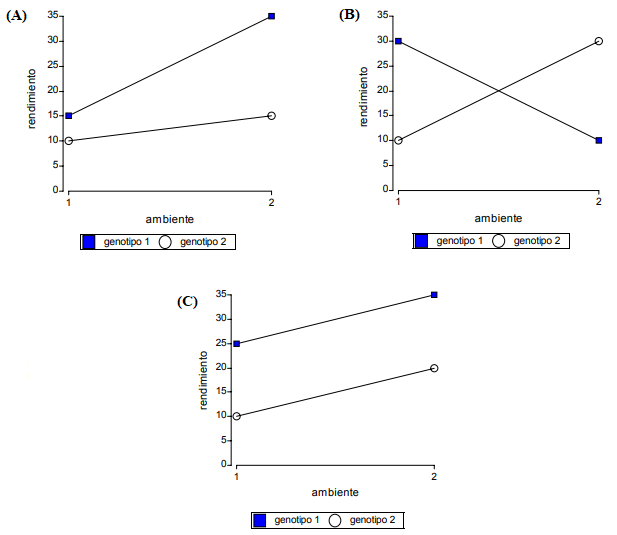
\includegraphics[width=14cm]{./Graficos/figura1}
\end{center}
\caption{Representación gráfica de tipos de IGA: (A)IGA no crossover, (B) IGA crossover y (C) no IGA}
\end{figure}


Distintos conceptos como regiones ecológicas, ecotipos, mega-ambientes, adaptaciones de germoplasma tanto en sentido amplio (a través de los ambientes) como específico (para cada ambiente o grupos de ambiente particular) (Kang et al., 2004) se pueden analizar a partir de la interacción genotipo-ambiente (Yan y Hunt, 2001).


Un análisis adecuado de la información de los EMA es indispensable para que el programa de mejoramiento de los cultivos sea eficaz. El rendimiento medio en los ambientes es un indicador suficiente del rendimiento genotípico solo en ausencia de IGA (Yan y Kang, 2003). Sin embargo, la aparición de IGA es inevitable y no basta con la comparación de las medias de los genotipos, sino que se debe recurrir a una metodología estadística más aporopiada. La metodología estadística más difundida para analizar los datos provenientes de EMA se basa en modificaciones de los modelos de regresión, análisis de variancia (\emph{Analysis of Variance}, ANOVA) y técnicas de análisis multivariado. 


Particularmente, para el estudio de la interacción y los análisis que de ella se derivan, dos modelos multiplicativos han aumentado su popularidad entre los fitomejoradores como una herramienta de análisis gráfico: el modelo de los efectos principales aditivos y interacción multiplicativa (AMMI, \emph{Additive Main effects and Multiplicative Interaction}) (Kempton 1984, Gauch, 1988), y el de regresión por sitio (SREG) (Cornelius et al., 1996; Crossa y Cornelius, 1997 y 2002).  Estos modelos combinan el análisis de varianza (ANOVA) y la descomposición de valores singulares (SVD) o el análisis de componentes principales (PCA) en la matriz residual de ANOVA. En SREG, el ANOVA se realiza sobre el efecto principal de A mientras que en AMMI se considera el efecto de G y A. A través del modelo AMMI se obtiene el gráfico biplot GE el cual es usado para explorar patrones puramente atribuibles a los efectos GE. Para el modelo SREG, Yan y Hunt (2002), presentaron la técnica GGE biplot usado para explorarnsimultáneamente patrones de variación en la suma G+GE.

Una limitación importante de la mayoría de las propuestas de análisis provenientes de EMA es que requieren que el conjunto de datos este completo. Aunque los EMA están diseñados para que todos los genotipos se evalúen en todos los ambientes,  las tablas de datos genotipo x ambiente completas son poco frecuentes (no todos los genotipos se encuentran en todos los ambientes). Esto ocurre, por ejemplo, debido a errores de medición o causas naturales como, por ejemplo, la destrucción de plantas por animales, inundaciones o durante la cosecha, la incorporación de nuevos genotipos y a que otros se descartan por su pobre desempeño (Hill y Rosemberg, 1985). En estos casos, entre las posibles soluciones para tratar con una tabla de datos incompleta es (i) el uso de un subconjunto completo de datos, eliminando aquellos genotipos que tienen valores faltantes (Ceccarelli et al., 2007, Yan et al., 2011), (ii) completar datos faltantes con la media ambiental, o (iii) imputación de datos faltantes con valores estimados utilizando, por ejemplo, un modelo multiplicativo (Kumar et al., 2012). 

En este contexto, el análisis de datos provenientes de EMA requiere metodología estadística sofisticada cuyas rutinas informáticas se encuentran disponibles en programas desarrollados por diferentes empresas. Esto genera el inconveniente de tener que disponer de todos los programas necesarios para los distintos análisis, atender los requerimientos de formatos de datos usados por cada uno, y comprender los diversos tipos de salidas en las que se ofrecen los resultados obtenidos. Además, algunos procedimientos, especialmente aquellas metodologías recientes, no se encuentran dispobibles, y los costos de las licencias de dichos programas resultan muy elevados. De aqui surge la necesidad de disponer de algún software libre que contemple la mayoría de las rutinas necesarias para analizar los datos provenientes de EMA. Este problema, puede ser resulto a partir del software R. Se trata de un proyecto de software libre distribuido bajo los términos de la \emph{General Public Licence} (GNU) que surge como resultado de la implementación de uno de los lenguajes más utilizados en investigación por la comunidad estadística, el lenguaje S. A diferencia de los programas estadísticos utilizados frecuentemente, R no dispone de una interfaz gráfica lo cual genera dificultad en su uso para aquellos que no se encuentran familiarizados con el uso de un lenguaje de programación. Sin embargo, brinda mayores posibilidades en cuanto a la manipulación y análisis de los datos ya lw permite a los usuarios definir sus propias funciones y  pesonalizar el tipo de análisis que desean realizar. 

R forma parte de un proyecto colaborativo ya que promueve el hecho de que los usuario creen funciones y las ponga al alcance de toda la comunidad.  Sin embargo, como muchas veces no resulta sencillo reutilizar una función creada por algun usuario se ha introducido la posibilidad de crear paquetes (\emph{package}) o librerías. Estas son una colección de objetos creados y organizados siguiendo un protocolo fijo que garantiza un soporte mínimo para el usuario así como la ausencia de errores (de sintaxis) en la programación.

R cuenta con 14 paquetes básicos y 29 recomendados para su funcionamiento instalados automaticamente en él, como por ejemplo, \emph{base} o \emph{stats}. Dado que la comunidad de usuarios que programan en R ha ido creciendo notablemente en los últimos años y que muchos de ellos han ido proporcionando librerías, se cuenta con una gran cantidad de paquetes que extienden las funciones básicas de R. Entre ellos se encuentran, \emph{plyr}, \emph{lubridate}, \emph{reshape2} y \emph{stringr} para la manipulación de los datos; \emph{ggplot2} y \emph{rgl} para la visualización; \emph{knitr} y \emph{xtable} para la presentación de resultados; entre otros. La lista completa de los paquetes oficiales puede consultarse en CRAN\footnote{CRAN (Comprehensive R Archve Network) es el repositorio oficial de paquetes de R, el lugar donde se publican las nuevas versiones del programa, etc. Contiene la lista completa de paquetes oficiales. \url{https://cran.r-project.org/web/packages/available_packages_by_name.html}}. Además de los paquetes oficiales, existen otros que pueden instalarse desde repositorios como, por ejemplo, Github. Sin embargo, no es sencillo encontrar un paquete que puede ser útil para un determinado fin sino que se debe recurrir a varios de ellos para cumplir un determinado objetivo. 

Frecuentemente, los mejoradores utilizan programas que tienen una interfaz gráfica para realizar los análisis estadísticos deseados y no tienen un manejo fluido de un lenguaje de programación. En el año 2012 se creó el paquete \emph{Shiny} que permite desarrollar aplicaciones Web utilizando R, acercando la potencia de R a todo tipo de usuarios.

El objetivo del presente trabajo fue: (i) crear un paquete de R que incluya las funciones que permitan analizar los datos provenientes de EMA, incluyendo además metodología recientemente publicada que no se encuentra disponible en R; (ii) crear una interfaz gráfica, entre R y el usuario, mediante Shiny con el fin de poder realizar los análisis disponibles en el paquete creado sin necesidad de utilizar el lenguaje de programación.



{\Huge{Pensar en hacer algun comentario de R studio}}
%% Los cap'itulos inician con \chapter{T'itulo}, estos aparecen numerados y
%% se incluyen en el 'indice general.
%%
%% Recuerda que aqu'i ya puedes escribir acentos como: 'a, 'e, 'i, etc.
%% La letra n con tilde es: 'n.
\chapter{Objetivos}
%\setcounter{section}{1}
\section{Objetivo general}
 
Desarrollar un paquete de R para el análisis de datos provenientes de EMA y una interfaza gráfica a través de la aplicación web Shiny.


\section{Objetivos específicos}
\begin{itemize}
\item Mostrar un flujo de trabajo reproducible para la construcción de paquetes de R.
\item Programar e incluir en el paquete de R metodología para el análisis de datos provenientes de EMA recientemente publicada y no disponible en R.
\item Añadir en el paquete de R funciones ya existentes con modificaciones o agregados para favorecer su uso.
\item Desarrollar una aplicación web Shiny que sirva como interfaz gráfica para el paquete.
\item Publicar el paquete y la aplicación para su libre uso.
\end{itemize}


%% Los cap'itulos inician con \chapter{T'itulo}, estos aparecen numerados y
%% se incluyen en el 'indice general.
%%
%% Recuerda que aqu'i ya puedes escribir acentos como: 'a, 'e, 'i, etc.
%% La letra n con tilde es: 'n.



\chapter{Métodos}
%\setcounter{section}{1}
\section{Paquete de R}

%https://oscarperpinan.github.io/R/Paquetes.html 
Una librería o paquete (\emph{package}) es una colección de objetos creados y organizados siguiendo un protocolo fijo que garantiza un soporte mínimo para el usuario así como la ausencia de errores (de sintaxis) en la programación.

\section{Creación del paquete de R}
Los pasos necesarios para la creación de un paquete son:
\begin{itemize}
\item Creación de los objetos que contendrá el paquete (funciones y/o
datos).
\item Creación del esqueleto del paquete.
\item Redacción de la documentación.
\item Compilación del paquete en Linux y creación de la versión para Windows.
\item Instalación.
\item Prueba y publicación.
\end{itemize}

\subsection{Objetos del paquete}
Un paquete puede contener cualquier tipo de objetos de R : funciones, datos etc. Lo primero que debe hacerse es programar las funciones y preparar los datos. El proceso de creación vigila que no hayan errores sintácticos pero no controla si hay errores lógicos.
 
\subsection{Esqueleto y estructura del paquete}
R proporciona una función \emph{package.skeleton} que permite automatizar el proceso de creación de un paquete creando los directorios, los archivos de documentación y otros objetos necesarios.
La  siguiente instrucción construye la estructura de un paquete llamado \emph{geneticae}, 

\begin{lstlisting}[frame=single]
package.skeleton(name = geneticae)
\end{lstlisting}

creando una carpeta de nombre \emph{geneticae} con 3 sub-carpetas en el directorio de trabajo y tres archivos sin extensión. Estos ultimos son los siguintes: 
\begin{itemize}

\item DESCRIPTION: contenido básico para
documentar según la descripción del paquete:

Package: geneticae\\
Type: Package\\
Title: What the package does (short line)\\
Version: 1.0\\
Date: 2019-09-21\\
Author: Who wrote it\\
Maintainer: Who to complain to <yourfault@somewhere.net>\\
Description: More about what it does (maybe more than one line)\\
License: What license is it under?\\

\item NAMESPACE: R usa un sistema de gestión de espacio de nombres que permite al autor del paquete especificar:
\begin{itemize}
\item las variables del paquete que se exportan (y son, por tanto, accesibles a los usuarios)
\item las variables que se importan de otros paquetes.
\item las clases y métodos S3 y S4 que deben registrarse.
\end{itemize}

Este mecanismo queda definido en el contenido del fichero NAMESPACE.

\item Read-and-delete-me: contiene algunas instrucciones importantes sobre cómo personalizar el paquete.
\end{itemize}

Las siguientes son las 3 sub-carpetas creadas:

\begin{itemize}
\item La carpeta \textbf{data} contiene todos los archivos correspondientes a los datos comprimidos con el nombre con el que fueron creados, con la extensión .rda. Estos no pueden ser modificados.
\item La carpeta \textbf{man} contiene todos los archivos de extensión .Rd y un archivo por objeto creado (datos o programa). Estos documentos son parte del sistema de ayuda del paquete en PDF y en HTML; por este motivo, la escritura sigue las reglas de LaTeX.
\item La carpeta \textbf{R} contiene todos los programas fuente, siendo .R la extensión de los mismos.
\end{itemize}
La documentación es uno de los aspectos mas importantes del código, sin ella, los usuarios no sabrán cómo usar el paquete. R proporciona una forma estándar de documentar paquetes: escribir archivos .Rd en la carpeta man, los cuales utilizan una sintaxis personalizada, basada en LaTeX. Sin embargo, el paquete \emph{roxygen2}, utilizado en este trabajo, permite obtener la documentación de una manera sencilla, proporcionando una serie de ventajas sobre la escritura los archivos .Rd:

\begin{itemize}
\item El código y la documentación son adyacentes, de modo que cuando el código se modifique, será fácil actualizar la documentación.

\item Inspecciona dinámicamente los objetos que está documentando, para que pueda agregar automáticamente los datos que de otra forma se deben escribir a mano.

\item Resume las diferencias en la documentación de los métodos S3 y S4, los genéricos y las clases, por lo que necesita aprender menos detalles.
\end{itemize}

Además de generar archivos .Rd, \emph{roxygen2} también creará un archivo NAMESPACE y administrará el campo \emph{Imports} del archivo DESCRIPTION.


\subsection{Compilación e instalación}
Una vez creada la documentación se debe chequear el paquete y generar los instaladores con su corresponiente manual. Para ello se utilizan las siguiente funciones:
\begin{itemize}
\item \emph{R CMD check} verificará que no haya errores de sintaxis o no se generen warnings. Está compuesto por más de 50 chequeos individuales entre los cuales se encuentran: la estructura del paquete, el archivo descripción, namespace, el código de R, los datos, la documentación, entre otros.
\item  \emph{R CMD build} compilará el paquete generando un archivo geneticae.tar.gz listo para su instalación en Linux y \emph{RCMD build -binary} generará el archivo para la instalación en Windows.
\item \emph{RCMD Rd2dvi --pdf} preparará el manual y \emph{R CMD INSTALL} instalará el paquete dejándolo listo para su uso
\end{itemize}

\subsection{Publicación}
%https://rsanchezs.gitbooks.io/ciencia-de-datos-con-r/paquetes/paquetes.html
Un repositorio es el lugar dónde están alojados los paquetes y desde el cuál se pueden descargarlos. Entre los repositorios más populares de paquetes R se encuentran:

\begin{itemize}
\item \textbf{CRAN}: es el principal repositorio de paquetes de R, está coordinado por la fundación R. Previa a la publicación en este repositorio el paquete debe pasar por diferentes pruebas para asegurar que cumple con las políticas de CRAN.

\item \textbf{Bioconductor}: se trata de un repositorio específico para bioinformática. Del mismo modo que CRAN, tiene sus propias políticas de publicaciones y procesos de revisión.

\item \textbf{GitHub}: a pesar que no es específico para R, github es con toda seguridad el repositorio más popular para la publicación de proyectos \emph{open source} (del inglés, código abierto). Su popularidad procede del espacio ilimitado que proporciona para el alojamiento de proyectos \emph{open source}, la integración con git (un software de control de versiones) y, la facilidad de compartir y colaborar con otras personas. Una de sus desventajas es que no proporciona procesos de control.

\item \textbf{R-Forge} y \textbf{RForge}: son entornos de desarrollo de paquetes y repositorios. Eso significa que incluyen control de fuente, seguimiento de errores y otras características. Puede obtener versiones de desarrollo de paquetes de estos.
\end{itemize}

El paquete \emph{geneticae} se encuentra en GitHub, para instalar el mismo (o cualquiera que se encuentre en dicho repositorio) se deben seguir las siguientes instrucciones:\\


\begin{lstlisting}[frame=single]
install.packages(remotes) 
library(remotes)
install_github(jangelini/geneticae) 
\end{lstlisting}


{\Huge{FALTAN LAS COMILLITAS EN INSTALL Y EN EL USUARIO DE GITHUB.. ME DA ERROR CUANDO LAS PONGO}}



{\Huge{(Ideas de: TRABAJO FINAL P SHINY)}}

\section{Aplicación Web}
Una aplicación web es una aplicación o herramienta informática accesible desde cualquier navegador, bien sea a través de internet (lo habitual) o bien a través de una red local. 
Estas aplicaciones son muy populares hoy en día para los usuarios no expertos, debido a la facilidad de su uso, ya que no es preciso instalar nada en el ordenador, simplemente se accede a través de un navegador. Además se puede acceder desde cualquier dispositivo con conexión a internet, ya sea un ordenador, un smartphone o una tablet, es decir que es independiente del sistema operativo del usuario. Otra gran ventaja es el bajo consumo de recursos, ya que la mayor parte del tiempo estos se consumen en el servidor donde se encuentra alojada la aplicación, que generalmente tiene mucha más potencia de cómputo que cualquier ordenador personal.

\section{Shiny APP}
%https://datanalytics.com/libro_r/shiny.html
Shiny es un paquete, que se encuentra instalado por defecto con Rstudio, con el que se pueden desarrollar aplicaciones web interactivas, directamente desde Rstudio sin necesitar conocimientos de HTML, CSS o Javascript. Shiny implementa la programación reactiva (cita de archivo aplicacion shiny) en donde los objetos (gráficos y tablas) que forman la aplicación responden a los inputs de los usuarios, dotando a estos de una gran capacidad de control.

En general, en estas aplicaciones, se distinguen tres pasos en el funcionamiento de la aplicación:
\begin{enumerate}
\item El usuario modifica todos aquellos widgets que quedan a su disposición en el navegador (los llamaremos inputs).
\item Los valores de los inputs se envían a R que realiza los análisis indicados.
\item Los resultados de estos cálculos se muestran en el navegador (los llamaremos outputs).
\end{enumerate}

El esquema interno de la aplicación puede observarse en la Figura \ref{fig:fig31}. 

\begin{figure}[h]
\begin{center}
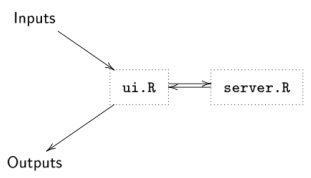
\includegraphics[width=7cm]{./Graficos/figura7}
\end{center}
\caption{Esquema interno de la aplicación.}
\label{fig:fig31}
\end{figure}


En las páginas y aplicaciones web se ha estandarizado el uso de ciertos lenguajes, tales como HTML, CSS, PHP o Javascript entre otros. Por defecto Shiny utiliza una plantilla básica de Twitter Bootstrap [18] para crear la interfaz de usuario, pero podemos descargar otras plantillas o crear una propia para personalizar nuestra aplicación. Twitter Bootstrap es un entorno de trabajo desarrollado por empleados de Twitter para fomentar la consistencia entre las herramientas internas, de forma que todas siguieran el mismo estilo. En 2011 Twitter liberó Bootstrap como código abierto, permitiendo que cualquiera lo usara para diseñar sus sitios o aplicaciones web. Contiene elementos de diseño basado en HTML, CSS y Javascript. Una de las mayores ventajas de Bootstrap es que permite crear interfaces web con CSS y JavaScript que adaptan la interfaz dependiendo del tamaño del dispositivo en el que se visualice de forma nativa, es decir, automáticamente se adapta al tamaño de un ordenador o de una tablet sin que el usuario tenga que hacer nada. Esto se denomina diseño adaptable o Responsive Design.

En lugar de usar un CSS propio para la interfaz de la aplicación se ha usado el paquete de R shinythemes [8], publicado por los creadores del propio Shiny. Shinytemes ofrece una serie de estilos básicos para aplicaciones Shiny.



\section{Creación de la Shiny APP}
%http://www.rpubs.com/JohanMarin/Shiny
La instalación de este paquete puede realizarse a través de los menús de Rstudio o simplemente con la siguiente orden:\\

\begin{lstlisting}[frame=single]
install.packages(shiny)
\end{lstlisting}

Para crear una Shiny app en \emph{File} se elige la opción Shiny Web App (figura \ref{fig:fig32}).

\begin{figure}[h]
\begin{center}
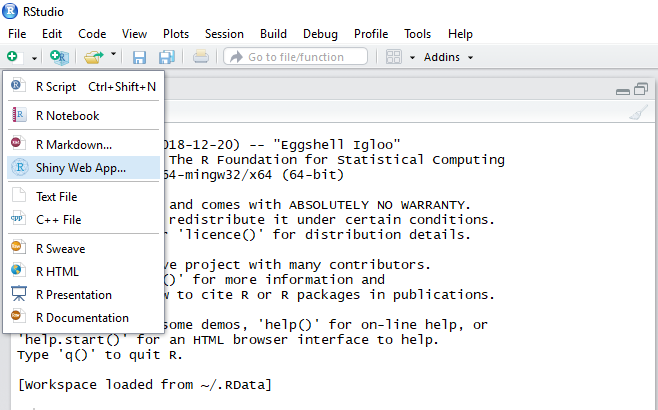
\includegraphics[width=12cm]{./Graficos/figura4}
\end{center}
\caption{Creación de Shiny Web App desde Rstudio}
\label{fig:fig32}
\end{figure}


Las aplicaciones Shiny están compuestas por un archivo app.R o dos archivos ui.R y server.R, es decir, se puede partir de un solo fichero que aglutine todo el código o se puede partir de dos archivos que separan la parte cliente de la parte servidora.

En este trabajo, se crea la aplicación Shiny mediante un unico script llamado app.R. El mismo se encuentra en un directorio (por ejemplo newdir/) y la aplicación se puede ejecutar con runApp(``newdir''). El script app.R esta formado por tres componentes:

\begin{itemize}
\item ui (\emph{user interfaz}): la interfaz de usuario controla el diseño de la aplicación, recibe los inputs y
muestra los outputs en el navegador.
\item server, funciones de R que contienen las instrucciones que se necesitan para construir los resultados de los análisis incluidos en la aplicación.
\item shinyApp, función que crea objetos de aplicación Shiny a partir de ui / servidor.
\end{itemize}


El archivo app.R deberá comenzar cargando el paquete Shiny y finalizar con una llamada a shinyApp:\\

\begin{lstlisting}[frame=single]
library(shiny)
ui<- ...
server<- ...
shinyApp(ui = ui, server = server)
\end{lstlisting}

La sesión de R estará monitoreando la aplicación y ejecutando las reacciones de la aplicación mientras la aplicación Shiny esté activa, por lo que no podrá ejecutar ningún comando.

La Figura \ref{fig:fig33} muestra el diseño utilizado en la aplicación. Se cuenta con un titulo y diferentes pestañas que conducen a diferentes páginas de la aplicación (\textbf{A}). Se cuenta con un panel de barra lateral (\textbf{B}), que contiene principalmente widgets con los cuales el usuario puede determinar el análisis que desea realizar y un panel principal (\textbf{C}) en el cual se obtenene los resultados del análisis solicitado.

\begin{figure}[h]
\begin{center}
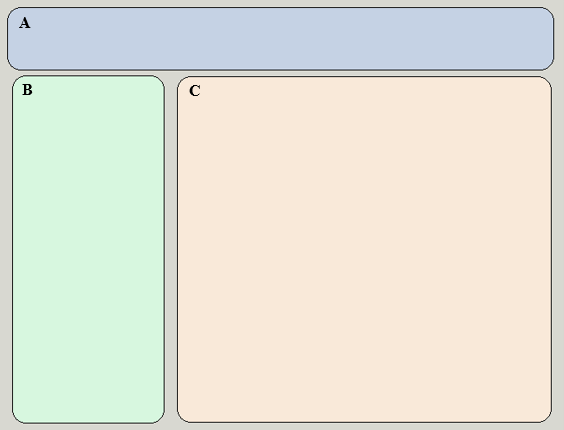
\includegraphics[width=12cm]{./Graficos/figura6}
\end{center}
\caption{Diseño de la aplicación Shiny. \textbf{A}: título y pestañas; \textbf{B}: área de entrada; \textbf{C}: área de resultados.}
\label{fig:fig33}
\end{figure}

\subsection{Tipos de componentes de Shiny Web App}

Los tipos de componentes de una aplación Shiny son:
\begin{itemize}
\item Componentes de Inputs y Outputs. Entre los inputs se encuentran numericInput, sliderInput, textInput, checkboxInput, entre otros. Posibles outputs se encuentran en la tabla \ref{tab:tabla1}, con las correspondientes funciones para server.R y ui.R
\item Componentes de Diseño. Algunos ejemplos se muestra en la tabla \ref{tab:tabla2}.
\item Componentes HTML (tags).
\end{itemize}


\begin{table}[h]
\begin{center}
\caption{Funciones para Outputs tanto para server.R como para ui.R}
\label{tab:tabla1}
\resizebox{\textwidth}{!} {
\begin{tabular}{cccc}
\hline
server.R & ui.R & espera & crea \\
\hline 
renderPlot & plotOutput & Gráfica & Gráfica\\
renderPrint & verbatimTextOutput, htmlOutput& salida impresa & texto\\
renderTable & tableOutput & objetos como tablas & tabla simple\\
renderDataTable & dataTableOutput & objetos como tablas & tabla DataTables.js\\
downloadHandler	& downloadButton, downloadLink & &\\
\hline 
\end{tabular}
}
\end{center}
\end{table}

\subsubsection{Componentes de Diseño}
% http://rstudio-pubs-static.s3.amazonaws.com/21373_8af3d3634b97461089c8a76659982915.html#componentes-shiny
\begin{itemize}
\item navbarPage(): Crea una página con una barra de navegación de nivel superior.
\item tabPanel(): Crea un panel de pestañas.
\item sidebarLayout(): Diseña de una barra lateral y el área principal.
\item sidebarPanel(): Crea un panel de barra lateral.
\item mainPanel(): Crea un panel principal.
\item navlistPanel(): Crea un panel de lista de navegación.
\item prettyRadioButtons(): Crea botones que permiten seleccionar un elemento de una lista.
\item materialSwitch(): Crea un interruptor de palanca para activar o desactivar una selección.
\item pickerInput(): Crea un control de selección de entrada.
\item navbarMenu():
\end{itemize}

{\small
\begin{table}[h]
\begin{center}
\caption{Componentes de Diseño de Shiny Web App}
\label{tab:tabla2}
\resizebox{0.6\textwidth}{!} {
\begin{tabular}{cccc}
\hline 
Componente	& Subcomponente	 \\
\hline
navbarPage(): & tabPanel(), navbarMenu()\\
navbarMenu() & tabPanel() \\
navlistPanel() & tabPanel()\\
titlePanel() &	\\
sidebarLayout() & sidebarPanel()  mainPanel() (obligatorio)	\\
sidebarPanel() & \\
mainPanel() & \\
tabsetPanel() &	\\
tabPanel()	 & \\
\hline
\end{tabular}
}
\end{center}
\end{table}
}


Para más información sobre estas componentes ver hoja de referencia de Shiny (Apéndice A).


\subsection{Compartiendo una Shiny Web App}

Una vez creada la aplicación, resulta conveniente ponerlas a disposición de los usuarios. En este caso la Shiny Web App encuentra disponible en el servidor de CONICET \url{www.cefobi.com}. Además el proyecto se encuentra en GitHub \url{https://github.com/jangelini/shinyAPP_geneticae}. 

%% Los cap'itulos inician con \chapter{T'itulo}, estos aparecen numerados y
%% se incluyen en el 'indice general.
%%
%% Recuerda que aqu'i ya puedes escribir acentos como: 'a, 'e, 'i, etc.
%% La letra n con tilde es: 'n.
\chapter{Resultados}
\section{Paquete de R \emph{geneticae}}

El paquete \emph{geneticae} ofrece funciones para el análisis de datos de etapas avanzadas de programas de mejoramiento, donde se evalúan pocos genotipos. 

Una vez que se instalado el paquete geneticae, se debe cargar en la sesion de R mediante el comando: \textcolor{blue}{library}(geneticae)

Es posible obtener información detallada sobre las funciones del paquete geneticae mediante de los archivos de ayuda indicando \textcolor{blue}{help}(package = "geneticae").  La ayuda para una función, por ejemplo, \textcolor{blue}{imputation}(), en una sesión R se puede obtener usando \emph{?imputation} o \textcolor{blue}{help}(imputation).


\subsection{Conjuntos de datos en geneticae}

El paquete geneticae proporciona dos conjuntos de datos para ilustrar la metodología incluida para analizar los datos MET.

\begin{itemize}
\item yan.winterwheat dataset: rendimiento de 18 variedades de trigo de invierno cultivadas en nueve ambientes en Ontario en 1993. No hay réplicas disponibles en los datos. Este conjunto de datos se obtuvo del paquete agridat.
\end{itemize}
\begin{lstlisting}
data(yan.winterwheat)
dat_yan <- yan.winterwheat
head(dat_yan)
\end{lstlisting}

\begin{verbatim}
##   gen  env yield
## 1 Ann BH93 4.460
## 2 Ari BH93 4.417
## 3 Aug BH93 4.669
## 4 Cas BH93 4.732
## 5 Del BH93 4.390
## 6 Dia BH93 5.178
\end{verbatim}
\begin{itemize}
\item plrv dataset: rendimiento, peso de planta y parcela de 28 clones de la población del virus del enrollamiento de la papa (PLRV) evaluada en seis entornos. Las réplicas están disponibles en los datos. Este conjunto de datos se obtuvo del paquete agricolae.
\end{itemize}
\begin{lstlisting}
data(plrv)
dat_rep <- plrv
head(dat_rep)
\end{lstlisting}


\begin{verbatim}
##   Genotype Locality Rep WeightPlant WeightPlot    Yield
## 1   102.18     Ayac   1   0.5100000       5.10 18.88889
## 2   104.22     Ayac   1   0.3450000       2.76 12.77778
## 3   121.31     Ayac   1   0.5425000       4.34 20.09259
## 4   141.28     Ayac   1   0.9888889       8.90 36.62551
## 5   157.26     Ayac   1   0.6250000       5.00 23.14815
## 6    163.9     Ayac   1   0.5120000       2.56 18.96296
\end{verbatim}

 
\subsection{Funciones en geneticae}

\textbf{Modelo de regresión por sitio}

Para ejecutar la función \textcolor{blue}{GGEmodel}(), se debe proporcionar un conjunto de datos con genotipos, ambientes, repeticiones (si hay disponibles), el fenotipo observado y los nombres que dichas variables tienen en el archivo de entrada. Además, se debe indicar el método de centrado, escala y SVD.

Cuando no hay repeticiones disponibles en el conjunto de datos, como es el caso del conjunto de datos yan.winterwheat, el modelo GGE se indica de la siguiente manera:


\begin{lstlisting}
GGE1 <- GGEmodel(dat_yan, genotype = "gen", environment = "env", response = "yield", centering = "tester")
\end{lstlisting}


Sin embargo, en el caso de que haya repeticiones disponibles, como el conjunto de datos plrv, se indica de la siguiente manera:


\begin{lstlisting}
GGE1_rep <- GGEmodel(dat_rep, genotype = "Genotype", environment = "Locality", response = "Yield", rep = "Rep", centering = "tester")
\end{lstlisting}


La salida de la función \textcolor{blue}{GGEmodel}() es una lista con los siguientes elementos:


\begin{itemize}
\item coordgenotype: trazado de coordenadas para genotipos de todos los componentes.
\item coordenviroment: trazado de coordenadas para entornos de todos los componentes.
\item valores propios: vector de valores propios de cada componente.
\item vartotal: varianza general.
\item varexpl: porcentaje de varianza explicado por cada componente.
\item labelgen: nombres de genotipo.
\item labelenv: nombres de entorno.
\item ejes: etiquetas de eje.
\item Datos: datos de entrada escalados y centrados.
\item centrado: nombre del método de centrado.
\item escala: nombre del método de escala.
\item SVP: nombre del método SVP.
\end{itemize}


Por ejemplo, para el conjunto de datos yan.winterwheat:


\begin{lstlisting}
names(GGE1)
\end{lstlisting}

\begin{verbatim}
##  [1] "coordgenotype"   "coordenviroment" "eigenvalues"    
##  [4] "vartotal"        "varexpl"         "labelgen"       
##  [7] "labelenv"        "labelaxes"       "Data"           
## [10] "centering"       "scaling"         "SVP"
\end{verbatim}


\textbf{Biplot GGE}

Para ejecutar la función \textcolor{blue}{GGEPlot}(), se requiere un objeto de la clase \textcolor{blue}{GGEmodel}(). La salida es un biplot construido a través de los componentes principales generados por \textcolor{blue}{GGEmodel}().

Los diferentes biplots que se pueden obtener usando la función \textcolor{blue}{GGEPlot}() se muestran usando el conjunto de datos yan.winterwheat. Si hay repeticiones disponibles en el conjunto de datos, como es el caso del conjunto plrv, se debe indicar el nombre de la columna que contiene las réplicas en el archivo de entrada.


\begin{itemize}
\item Biplot básico

\begin{lstlisting}
GGEPlot(GGE1, type = "Biplot")
\end{lstlisting}

\begin{figure}[H]
	\begin{center}
		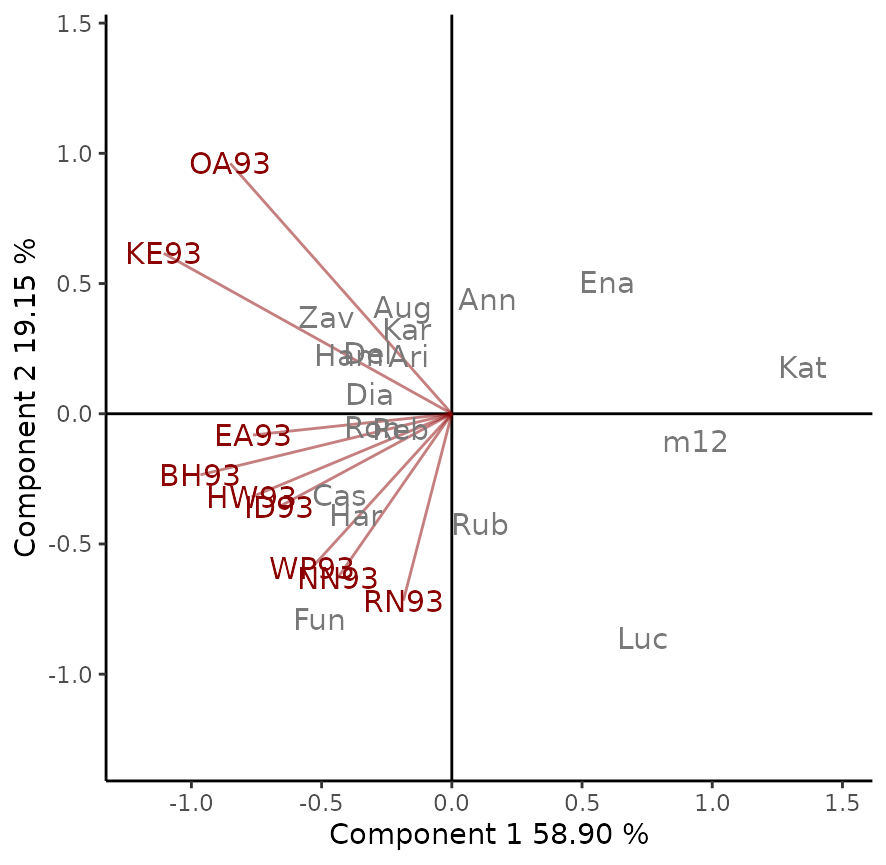
\includegraphics[width=10cm]{./Graficos/GGE_BIPLOT.png}
	\end{center}
	\caption{Biplot básico obtenido de la función \textcolor{blue}{GGEPlot}()}
\end{figure}

\item Ranking de los cultivares en función de su rendimiento en el ambiente OA93.

\begin{lstlisting}
GGEPlot(GGE1, type = "Selected Environment", selectedE = "OA93")
\end{lstlisting}


\begin{figure}[H]
	\begin{center}
		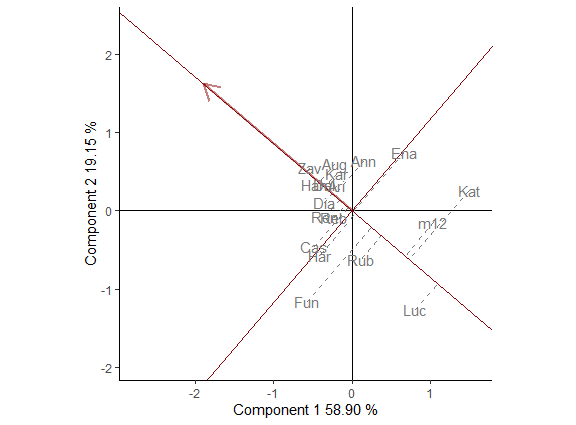
\includegraphics[width=10cm]{./Graficos/SelectedEnvironment.png}
	\end{center}
	\caption{Ranking de cultivares para un ambiente determinado obtenido de la función \textcolor{blue}{GGEPlot}()}
\end{figure}


\item Ranking de los ambientes en función del rendimiento relativo del cultivar Kat.

\begin{lstlisting}
GGEPlot(GGE1, type = "Selected Genotype", selectedG = "Kat")
\end{lstlisting}

\begin{figure}[H]
	\begin{center}
		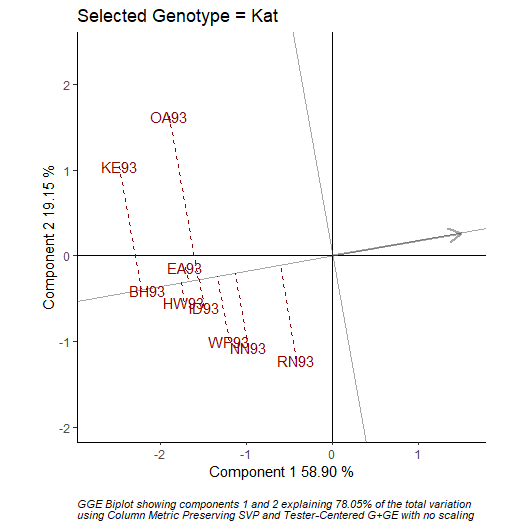
\includegraphics[width=10cm]{./Graficos/SelectedGenotype.png}
	\end{center}
	\caption{Ranking de ambientes para cultivar determinado obtenido de la función \textcolor{blue}{GGEPlot}()}
\end{figure}


\item Relación entre ambientes.

\begin{lstlisting}
GGEPlot(GGE1, type = "Relationship Among Environments")
\end{lstlisting}

\begin{figure}[H]
	\begin{center}
		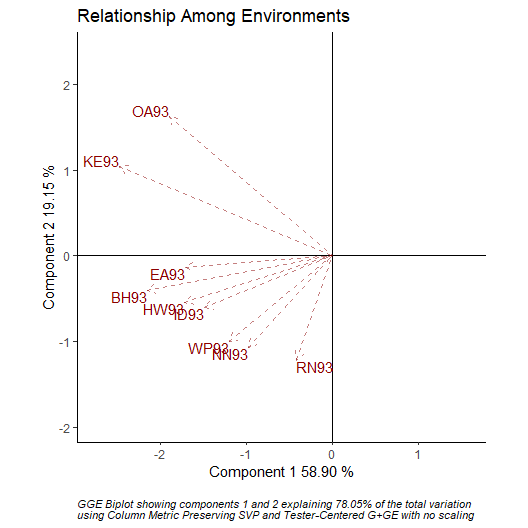
\includegraphics[width=10cm]{./Graficos/RelationshipAmongEnvironments.png}
	\end{center}
	\caption{Relación entre ambientes obtenido de la función \textcolor{blue}{GGEPlot}()}
\end{figure}

\item Comparación entre los genotipos Kat y Cas.

\begin{lstlisting}
GGEPlot(GGE1, type = "Comparison of Genotype", selectedG1 = "Kat", selectedG2 = "Cas")
\end{lstlisting}

\begin{figure}[H]
	\begin{center}
		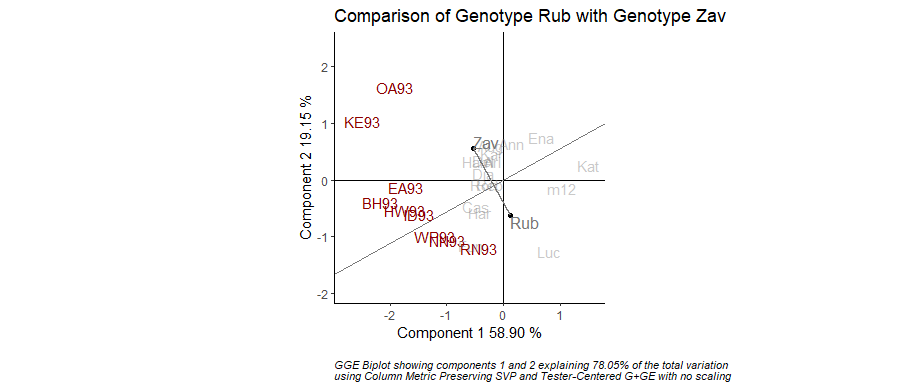
\includegraphics[width=10cm]{./Graficos/ComparisonofGenotype.png}
	\end{center}
	\caption{Comparación entre dos genotipos obtenido de la función \textcolor{blue}{GGEPlot}()}
\end{figure}


\item Identificación del mejor cultivar en cada ambiente.

\begin{lstlisting}
GGEPlot(GGE1, type = "Which Won Where/What")
\end{lstlisting}

\begin{figure}[H]
	\begin{center}
		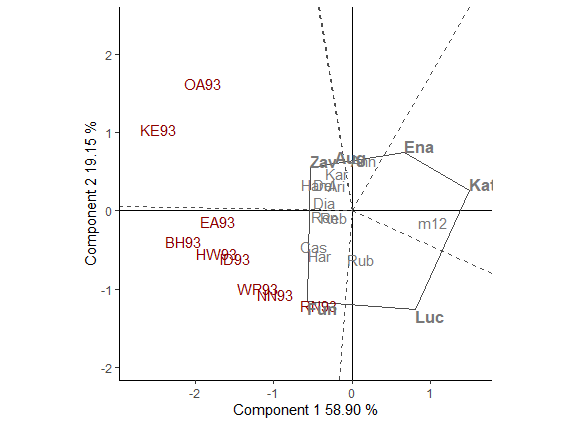
\includegraphics[width=12cm]{./Graficos/WhichWonWhereWhat.png}
	\end{center}
	\caption{Identificación del mejor cultivar en cada ambiente a partir de la función \textcolor{blue}{GGEPlot}()}
\end{figure}



\item Evaluación de los ambientes basados tanto en la capacidad de discriminación como en la representatividad.

\begin{lstlisting}
GGEPlot(GGE1, type = "Discrimination vs. representativeness")
\end{lstlisting}

\begin{figure}[H]
	\begin{center}
		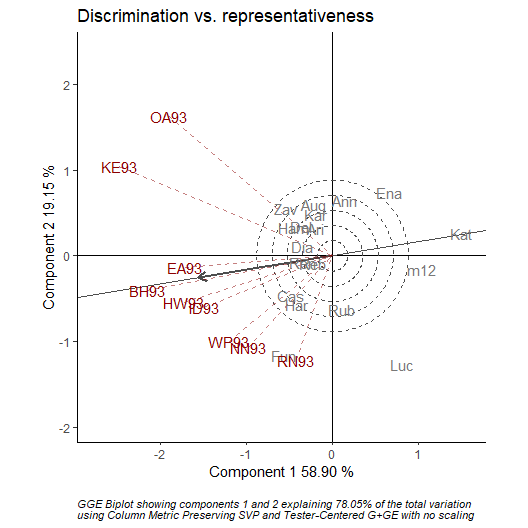
\includegraphics[width=12cm]{./Graficos/Discriminationvsrepresentativeness.png}
	\end{center}
	\caption{Evaluación de los ambientes basados tanto en la capacidad de discriminación y representatividad a partir de la función \textcolor{blue}{GGEPlot}()}
\end{figure}



\item Clasificación de ambientes con respecto al ambiente ideal.

\begin{lstlisting}
GGEPlot(GGE1, type = "Ranking Environments")
\end{lstlisting}

\begin{figure}[H]
	\begin{center}
		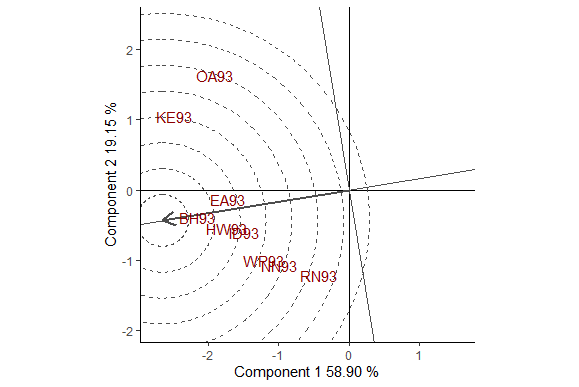
\includegraphics[width=12cm]{./Graficos/RankingEnvironments.png}
	\end{center}
	\caption{Clasificación de ambientes con respecto al ambiente ideal a partir de la función \textcolor{blue}{GGEPlot}()}
\end{figure}


\item Clasificación de genotipos con respecto al genotipo ideal.

\begin{lstlisting}
GGEPlot(GGE1, type = "Ranking Genotypes")
\end{lstlisting}

\begin{figure}[H]
	\begin{center}
		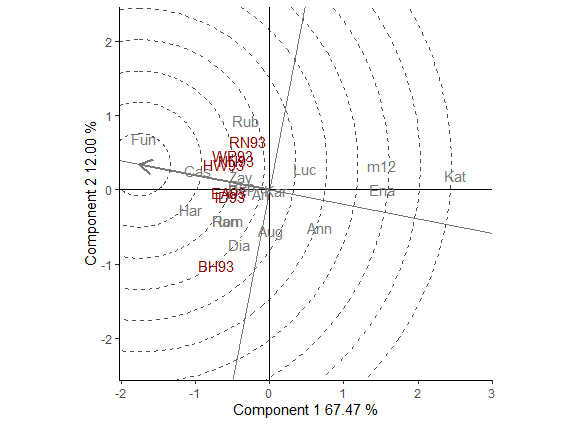
\includegraphics[width=10cm]{./Graficos/RankingGenotypes.png}
	\end{center}
	\caption{Clasificación de genotipos con respecto al genotipo ideal a partir de la función \textcolor{blue}{GGEPlot}()}
\end{figure}

\item Evaluación de los cultivares con base en el rendimiento promedio y la estabilidad.

\begin{lstlisting}
GGEPlot(GGE1, type = "Mean vs. Stability")
\end{lstlisting}

\begin{figure}[H]
	\begin{center}
		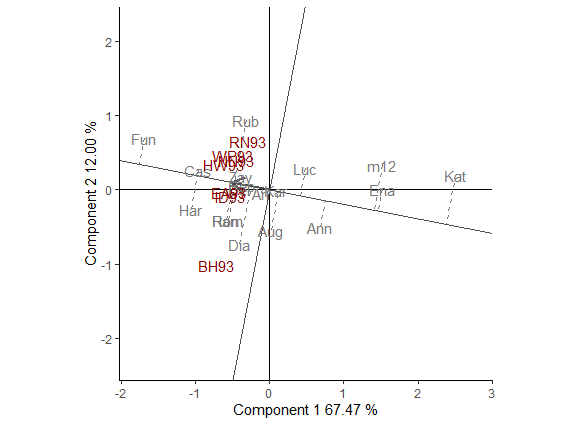
\includegraphics[width=10cm]{./Graficos/MeanvsStability.png}
	\end{center}
	\caption{Evaluación de los cultivares con base en el rendimiento promedio y la estabilidad a partir de la función \textcolor{blue}{GGEPlot}()}
\end{figure}

\end{itemize}


\textbf{Classic AMMI model}

Para ejecutar la función \textcolor{blue}{rAMMI}(), como en la función \textcolor{blue}{GGEmodel}(), se debe proporcionar un conjunto de datos con genotipo, entorno, repeticiones (si las hay) y la variable de respuesta. Se debe indicar el nombre de las columnas que contienen cada una de estas variables en el conjunto de datos de entradas. La salida de la función es un biplot.

A continuación se muestra el biplot GE obtenido del modelo AMMI clásico obtenido con el conjunto de datos yan.winterwheat.

\begin{lstlisting}
rAMMI(dat_yan, genotype = "gen", environment = "env", response = "yield", type = "AMMI")
\end{lstlisting}

\begin{figure}[H]
	\begin{center}
		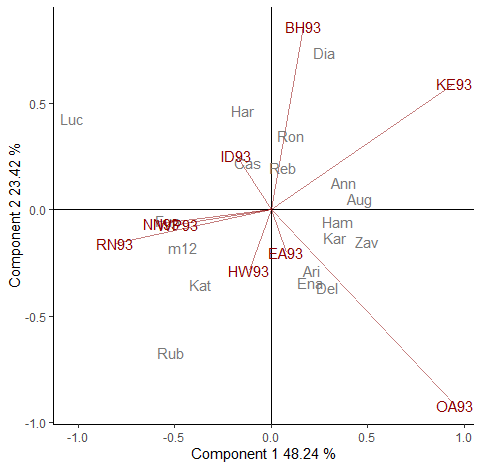
\includegraphics[width=10cm]{./Graficos/AMMI.png}
	\end{center}
	\caption{Biplot GE obtenido del modelo clasico AMMI}
\end{figure}

\textbf{Robust AMMI model}

Como se dijo anteriormente, el modelo AMMI clasico, en su forma estándar, no funciona bien en presencia de observaciones atípicas. Dado que los outliers son muy comun en los datos agronómicos, Rodrigues et al. (2015) proponen cinco modelos AMMI robustos, que permiten superar el problema de la contaminación de datos con observaciones atípicas. Los biplots de los cinco modelos AMMI robustos propuestos por Rodrigues et al. (2015), se pueden obtener utilizando la función \textcolor{blue}{rAMMI}() A continuación se muestran los biplots obtenidos con dichos modelos robustos usando el conjunto de datos yan.winterwheat.

\begin{itemize}

\item  modelo "rAMMI"

\begin{lstlisting}
rAMMI(dat_yan, genotype = "gen", environment = "env", response = "yield", type = "rAMMI")
\end{lstlisting}

\begin{figure}[H]
	\begin{center}
		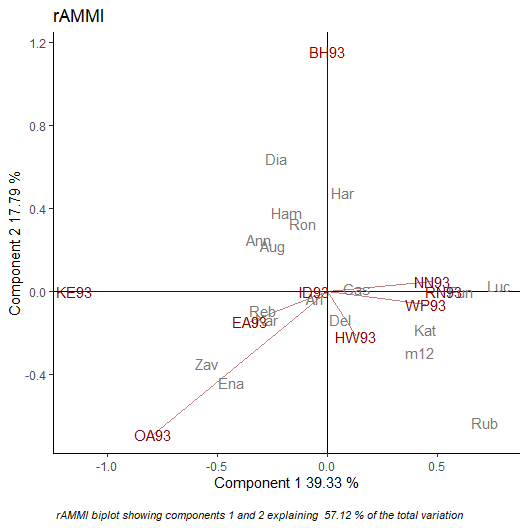
\includegraphics[width=10cm]{./Graficos/rAMMI.png}
	\end{center}
	\caption{Biplot GE obtenido del modelo robusto rAMMI}
\end{figure}


\item  modelo "hAMMI"

\begin{lstlisting}
rAMMI(dat_yan, genotype = "gen", environment = "env", response = "yield", type = "hAMMI")
\end{lstlisting}

\begin{figure}[H]
	\begin{center}
		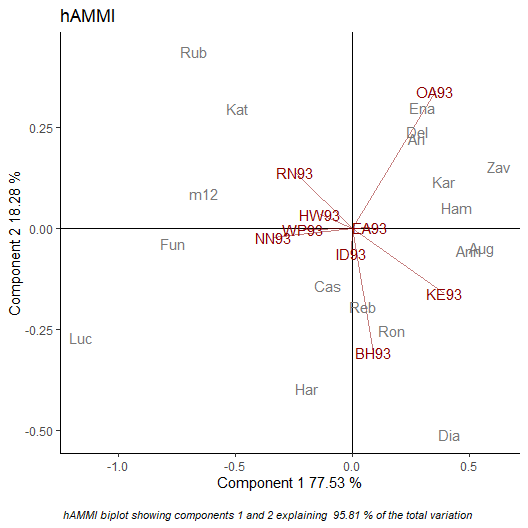
\includegraphics[width=10cm]{./Graficos/hAMMI.png}
	\end{center}
	\caption{Biplot GE obtenido del modelo robusto hAMMI}
\end{figure}


\item  modelo "gAMMI"

\begin{lstlisting}
rAMMI(dat_yan, genotype = "gen", environment = "env", response = "yield", type = "gAMMI")
\end{lstlisting}

\begin{figure}[H]
	\begin{center}
		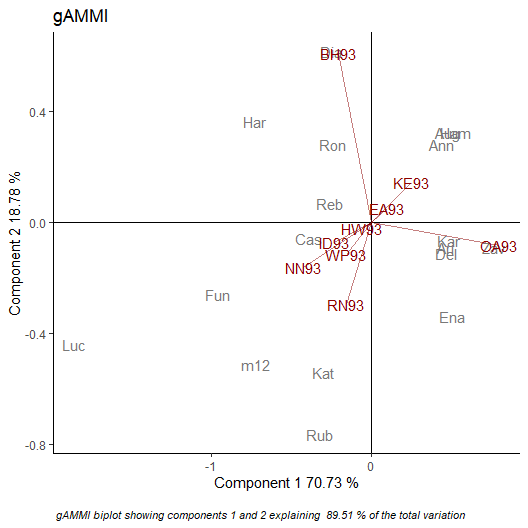
\includegraphics[width=10cm]{./Graficos/gAMMI.png}
	\end{center}
	\caption{Biplot GE obtenido del modelo robusto gAMMI}
\end{figure}



\item  modelo "lAMMI"

\begin{lstlisting}
rAMMI(dat_yan, genotype = "gen", environment = "env", response = "yield", type = "lAMMI")
\end{lstlisting}


\begin{figure}[H]
	\begin{center}
		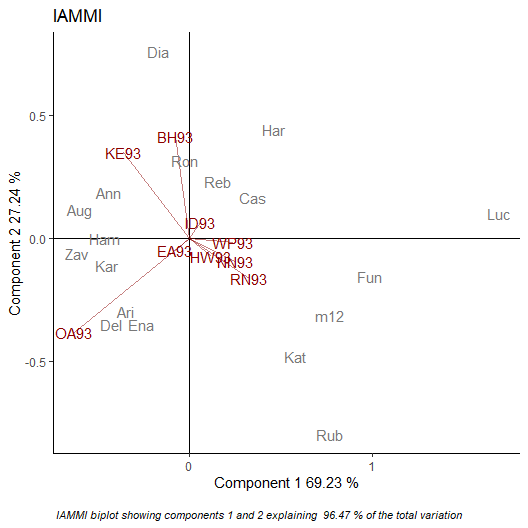
\includegraphics[width=10cm]{./Graficos/lAMMI.png}
	\end{center}
	\caption{Biplot GE obtenido del modelo robusto lAMMI}
\end{figure}


\item  modelo "ppAMMI"
\begin{lstlisting}
rAMMI(dat_yan, genotype = "gen", environment = "env", response = "yield", type = "ppAMMI")
\end{lstlisting}


\begin{figure}[H]
	\begin{center}
		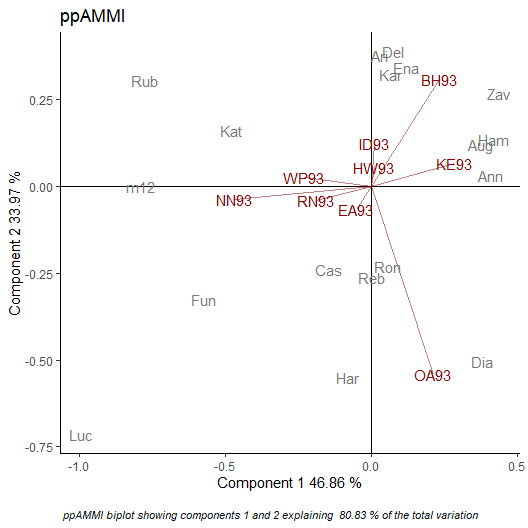
\includegraphics[width=10cm]{./Graficos/ppAMMI.png}
	\end{center}
	\caption{Biplot GE obtenido del modelo robusto ppAMMI}
\end{figure}

\end{itemize}

\textbf{Métodos de imputación}
Una limitación importante de los modelos presentados anteriormente es que requieren una que el conjunto de datos este completo. Por lo tanto, en el paquete se incluyen una serie de metodologías propuestas, algunas de las cuales no se encuentran disponible en R, para superar el problema de falta de equilibrio. 

El conjunto de datos yan.winterwheat se utilizó como ejemplo. Como el conjunto de datos no contaba con observaciones perdidas, algunas fueron eliminadas con el objetivo de mostrar las metodologías de imputación incluidas.

\begin{lstlisting}
# generates missing data
dat_yan[1, 3] <- NA
dat_yan[3, 3] <- NA
dat_yan[2, 3] <- NA
\end{lstlisting}


\begin{itemize}
\item GabrielEigein proposed by Arciniegas-Alarcón S., et al. (2010).
\end{itemize}
\begin{lstlisting}
imputation(dat_yan, PC.nb = 2, genotype = "gen", environment = "env", response = "yield", type = "EM-AMMI")
\end{lstlisting}
\centering
\begin{small}
\begin{Verbatim}[frame=single,baselinestretch=0.3]
##         BH93  EA93  HW93  ID93  KE93  NN93  OA93  RN93  WP93
## Ann 4.150120 4.150 2.849 3.084 5.940 4.450 4.351 4.039 2.672
## Ari 4.035814 4.771 2.912 3.506 5.699 5.152 4.956 4.386 2.938
## Aug 4.305244 4.578 3.098 3.460 6.070 5.025 4.730 3.900 2.621
## Cas 4.732000 4.745 3.375 3.904 6.224 5.340 4.226 4.893 3.451
## Del 4.390000 4.603 3.511 3.848 5.773 5.421 5.147 4.098 2.832
## Dia 5.178000 4.475 2.990 3.774 6.583 5.045 3.985 4.271 2.776
## Ena 3.375000 4.175 2.741 3.157 5.342 4.267 4.162 4.063 2.032
## Fun 4.852000 4.664 4.425 3.952 5.536 5.832 4.168 5.060 3.574
## Ham 5.038000 4.741 3.508 3.437 5.960 4.859 4.977 4.514 2.859
## Har 5.195000 4.662 3.596 3.759 5.937 5.345 3.895 4.450 3.300
## Kar 4.293000 4.530 2.760 3.422 6.142 5.250 4.856 4.137 3.149
## Kat 3.151000 3.040 2.388 2.350 4.229 4.257 3.384 4.071 2.103
## Luc 4.104000 3.878 2.302 3.718 4.555 5.149 2.596 4.956 2.886
## Reb 4.375000 4.701 3.655 3.592 6.189 5.141 3.933 4.208 2.925
## Ron 4.940000 4.698 2.950 3.898 6.063 5.326 4.302 4.299 3.031
## Rub 3.786000 4.969 3.379 3.353 4.774 5.304 4.322 4.858 3.382
## Zav 4.238000 4.654 3.607 3.914 6.641 4.830 5.014 4.363 3.111
## m12 3.340000 3.854 2.419 2.783 4.629 5.090 3.281 3.918 2.561
\end{Verbatim}
\end{small}


\begin{itemize}
\item EM-AMMI proposed by Gauch and Zobel (1990).
\end{itemize}
\begin{lstlisting}
imputation(dat_yan, PC.nb = 1, genotype = "gen", environment = "env", response = "yield", type = "EM-AMMI")
\end{lstlisting}

\begin{verbatim}
##         BH93  EA93  HW93  ID93  KE93  NN93  OA93  RN93  WP93
## Ann 4.136249 4.150 2.849 3.084 5.940 4.450 4.351 4.039 2.672
## Ari 4.474249 4.771 2.912 3.506 5.699 5.152 4.956 4.386 2.938
## Aug 4.386299 4.578 3.098 3.460 6.070 5.025 4.730 3.900 2.621
## Cas 4.732000 4.745 3.375 3.904 6.224 5.340 4.226 4.893 3.451
## Del 4.390000 4.603 3.511 3.848 5.773 5.421 5.147 4.098 2.832
## Dia 5.178000 4.475 2.990 3.774 6.583 5.045 3.985 4.271 2.776
## Ena 3.375000 4.175 2.741 3.157 5.342 4.267 4.162 4.063 2.032
## Fun 4.852000 4.664 4.425 3.952 5.536 5.832 4.168 5.060 3.574
## Ham 5.038000 4.741 3.508 3.437 5.960 4.859 4.977 4.514 2.859
## Har 5.195000 4.662 3.596 3.759 5.937 5.345 3.895 4.450 3.300
## Kar 4.293000 4.530 2.760 3.422 6.142 5.250 4.856 4.137 3.149
## Kat 3.151000 3.040 2.388 2.350 4.229 4.257 3.384 4.071 2.103
## Luc 4.104000 3.878 2.302 3.718 4.555 5.149 2.596 4.956 2.886
## Reb 4.375000 4.701 3.655 3.592 6.189 5.141 3.933 4.208 2.925
## Ron 4.940000 4.698 2.950 3.898 6.063 5.326 4.302 4.299 3.031
## Rub 3.786000 4.969 3.379 3.353 4.774 5.304 4.322 4.858 3.382
## Zav 4.238000 4.654 3.607 3.914 6.641 4.830 5.014 4.363 3.111
## m12 3.340000 3.854 2.419 2.783 4.629 5.090 3.281 3.918 2.561
\end{verbatim}



\begin{itemize}
\item EM-SVD proposed by Perry (2009)
\end{itemize}
\begin{lstlisting}
imputation(dat_yan, genotype = "gen", environment = "env", response = "yield", type = "EM-SVD")
\end{lstlisting}

\begin{verbatim}
##           [,1]  [,2]  [,3]  [,4]  [,5]  [,6]  [,7]  [,8]  [,9]
##  [1,] 4.332467 4.150 2.849 3.084 5.940 4.450 4.351 4.039 2.672
##  [2,] 4.332467 4.771 2.912 3.506 5.699 5.152 4.956 4.386 2.938
##  [3,] 4.332467 4.578 3.098 3.460 6.070 5.025 4.730 3.900 2.621
##  [4,] 4.732000 4.745 3.375 3.904 6.224 5.340 4.226 4.893 3.451
##  [5,] 4.390000 4.603 3.511 3.848 5.773 5.421 5.147 4.098 2.832
##  [6,] 5.178000 4.475 2.990 3.774 6.583 5.045 3.985 4.271 2.776
##  [7,] 3.375000 4.175 2.741 3.157 5.342 4.267 4.162 4.063 2.032
##  [8,] 4.852000 4.664 4.425 3.952 5.536 5.832 4.168 5.060 3.574
##  [9,] 5.038000 4.741 3.508 3.437 5.960 4.859 4.977 4.514 2.859
## [10,] 5.195000 4.662 3.596 3.759 5.937 5.345 3.895 4.450 3.300
## [11,] 4.293000 4.530 2.760 3.422 6.142 5.250 4.856 4.137 3.149
## [12,] 3.151000 3.040 2.388 2.350 4.229 4.257 3.384 4.071 2.103
## [13,] 4.104000 3.878 2.302 3.718 4.555 5.149 2.596 4.956 2.886
## [14,] 4.375000 4.701 3.655 3.592 6.189 5.141 3.933 4.208 2.925
## [15,] 4.940000 4.698 2.950 3.898 6.063 5.326 4.302 4.299 3.031
## [16,] 3.786000 4.969 3.379 3.353 4.774 5.304 4.322 4.858 3.382
## [17,] 4.238000 4.654 3.607 3.914 6.641 4.830 5.014 4.363 3.111
## [18,] 3.340000 3.854 2.419 2.783 4.629 5.090 3.281 3.918 2.561
\end{verbatim}


\begin{itemize}
\item WGabriel proposed by Alarcon…..
\end{itemize}
\begin{lstlisting}
imputation(dat_yan, genotype = "gen", environment = "env", response = "yield", type = "WGabriel")
\end{lstlisting}

\begin{verbatim}
##         BH93  EA93  HW93  ID93  KE93  NN93  OA93  RN93  WP93
## Ann 4.004664 4.150 2.849 3.084 5.940 4.450 4.351 4.039 2.672
## Ari 4.455727 4.771 2.912 3.506 5.699 5.152 4.956 4.386 2.938
## Aug 4.328095 4.578 3.098 3.460 6.070 5.025 4.730 3.900 2.621
## Cas 4.732000 4.745 3.375 3.904 6.224 5.340 4.226 4.893 3.451
## Del 4.390000 4.603 3.511 3.848 5.773 5.421 5.147 4.098 2.832
## Dia 5.178000 4.475 2.990 3.774 6.583 5.045 3.985 4.271 2.776
## Ena 3.375000 4.175 2.741 3.157 5.342 4.267 4.162 4.063 2.032
## Fun 4.852000 4.664 4.425 3.952 5.536 5.832 4.168 5.060 3.574
## Ham 5.038000 4.741 3.508 3.437 5.960 4.859 4.977 4.514 2.859
## Har 5.195000 4.662 3.596 3.759 5.937 5.345 3.895 4.450 3.300
## Kar 4.293000 4.530 2.760 3.422 6.142 5.250 4.856 4.137 3.149
## Kat 3.151000 3.040 2.388 2.350 4.229 4.257 3.384 4.071 2.103
## Luc 4.104000 3.878 2.302 3.718 4.555 5.149 2.596 4.956 2.886
## Reb 4.375000 4.701 3.655 3.592 6.189 5.141 3.933 4.208 2.925
## Ron 4.940000 4.698 2.950 3.898 6.063 5.326 4.302 4.299 3.031
## Rub 3.786000 4.969 3.379 3.353 4.774 5.304 4.322 4.858 3.382
## Zav 4.238000 4.654 3.607 3.914 6.641 4.830 5.014 4.363 3.111
## m12 3.340000 3.854 2.419 2.783 4.629 5.090 3.281 3.918 2.561
\end{verbatim}

\begin{itemize}
\item EM-PCA proposed by
\end{itemize}
\begin{lstlisting}
imputation(dat_yan, genotype = "gen", environment = "env", response = "yield", type = "EM-PCA")
\end{lstlisting}

\begin{verbatim}
##         BH93  EA93  HW93  ID93  KE93  NN93  OA93  RN93  WP93
## Ann 3.980317 4.150 2.849 3.084 5.940 4.450 4.351 4.039 2.672
## Ari 4.463093 4.771 2.912 3.506 5.699 5.152 4.956 4.386 2.938
## Aug 4.327731 4.578 3.098 3.460 6.070 5.025 4.730 3.900 2.621
## Cas 4.732000 4.745 3.375 3.904 6.224 5.340 4.226 4.893 3.451
## Del 4.390000 4.603 3.511 3.848 5.773 5.421 5.147 4.098 2.832
## Dia 5.178000 4.475 2.990 3.774 6.583 5.045 3.985 4.271 2.776
## Ena 3.375000 4.175 2.741 3.157 5.342 4.267 4.162 4.063 2.032
## Fun 4.852000 4.664 4.425 3.952 5.536 5.832 4.168 5.060 3.574
## Ham 5.038000 4.741 3.508 3.437 5.960 4.859 4.977 4.514 2.859
## Har 5.195000 4.662 3.596 3.759 5.937 5.345 3.895 4.450 3.300
## Kar 4.293000 4.530 2.760 3.422 6.142 5.250 4.856 4.137 3.149
## Kat 3.151000 3.040 2.388 2.350 4.229 4.257 3.384 4.071 2.103
## Luc 4.104000 3.878 2.302 3.718 4.555 5.149 2.596 4.956 2.886
## Reb 4.375000 4.701 3.655 3.592 6.189 5.141 3.933 4.208 2.925
## Ron 4.940000 4.698 2.950 3.898 6.063 5.326 4.302 4.299 3.031
## Rub 3.786000 4.969 3.379 3.353 4.774 5.304 4.322 4.858 3.382
## Zav 4.238000 4.654 3.607 3.914 6.641 4.830 5.014 4.363 3.111
## m12 3.340000 3.854 2.419 2.783 4.629 5.090 3.281 3.918 2.561
\end{verbatim}


\section{Geneticae Shiny Web App}

La aplicación Geneticae se organiza en las siguientes pestañas:
\begin{itemize}
\item Los datos
\item Análisis descriptivo
\item ANOVA
\item Biplot GGE
\item Biplot GE
\item Ayuda
\end{itemize}

En muchos casos, algunos atributos estilísticos de salida pueden personalizarse para que el usuario obtenga la salida a su gusto. A su vez, los gráficos obtenidos pueden ser descargados.

\subsection{Los datos}
Al iniciar la aplicación Geneticae, se muestra una pantalla en la cual se carga el conjunto de datos a analizar. La aplicación admite datos en formato .csv, delimitados por coma o punto y coma; y también acepta la primera fila como encabezado. La aplicación puede leer un tipo de formato de datos: 
\begin{itemize}
\item Cada fila contiene una observación, que se compone de tres o cuatro valores: nombre del cultivar, ambiente, repetición si \item está disponible y valor fenotipico medido.
\item La primera fila de encabezado contiene los nombres de cada variable. Los encabezados pueden dar cualquier nombre que elija, y deben indicarse al cargar el archivo de datos.
\item El número de repeticiones puede diferir con los genotipos y los entornos.
\end{itemize}

Se utilizan dos conjuntos de datos, incluidos en el paquete Geneticae, para ilustrar la aplicación. Estos conjuntos de datos, uno de los cuales tiene repeticiones (conjunto de datos plrv) y el otro no (conjunto de datos yang), los cuales se pueden ver y descargar en la pestaña \emph{The data} $\rightarrow$ \emph{Example datasets} (Figura \ref{fig:fig41},\ref{fig:fig42}). 

\begin{figure}[H]
	\begin{center}
		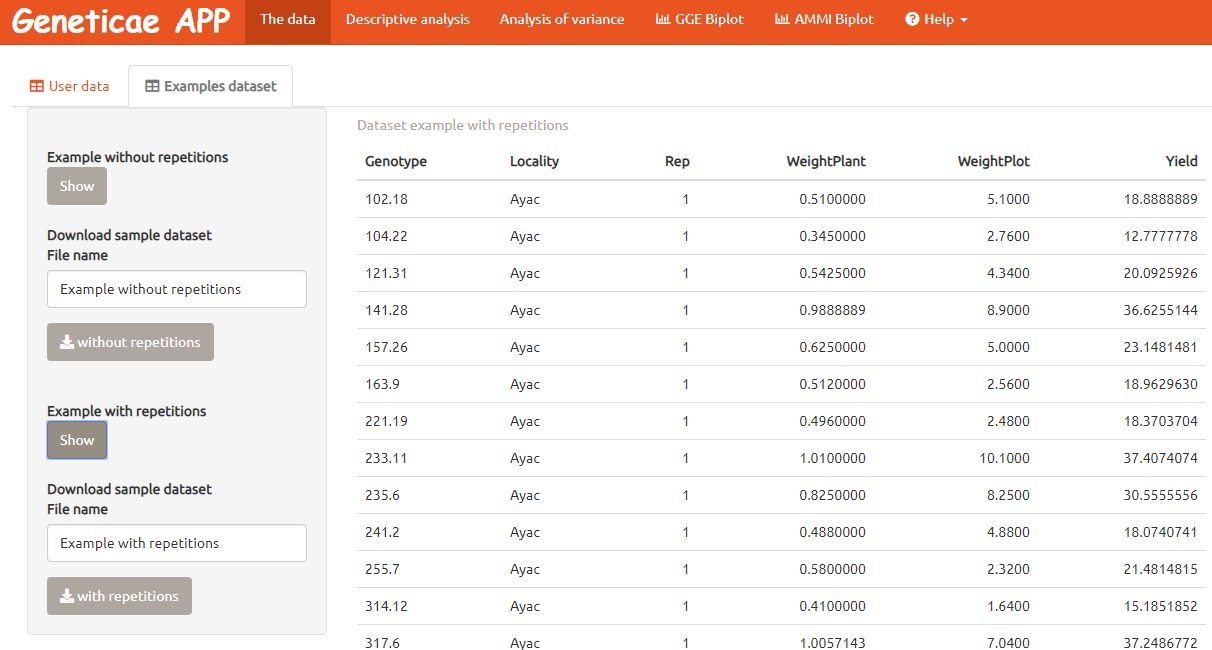
\includegraphics[width=17cm]{./Graficos/Exampledatasets_withoutrep.png}
	\end{center}
	\caption{Conjunto de datos sin repetición disponible en Shiny Web App}
	\label{fig:fig41}
\end{figure}


\begin{figure}[H]
	\begin{center}
		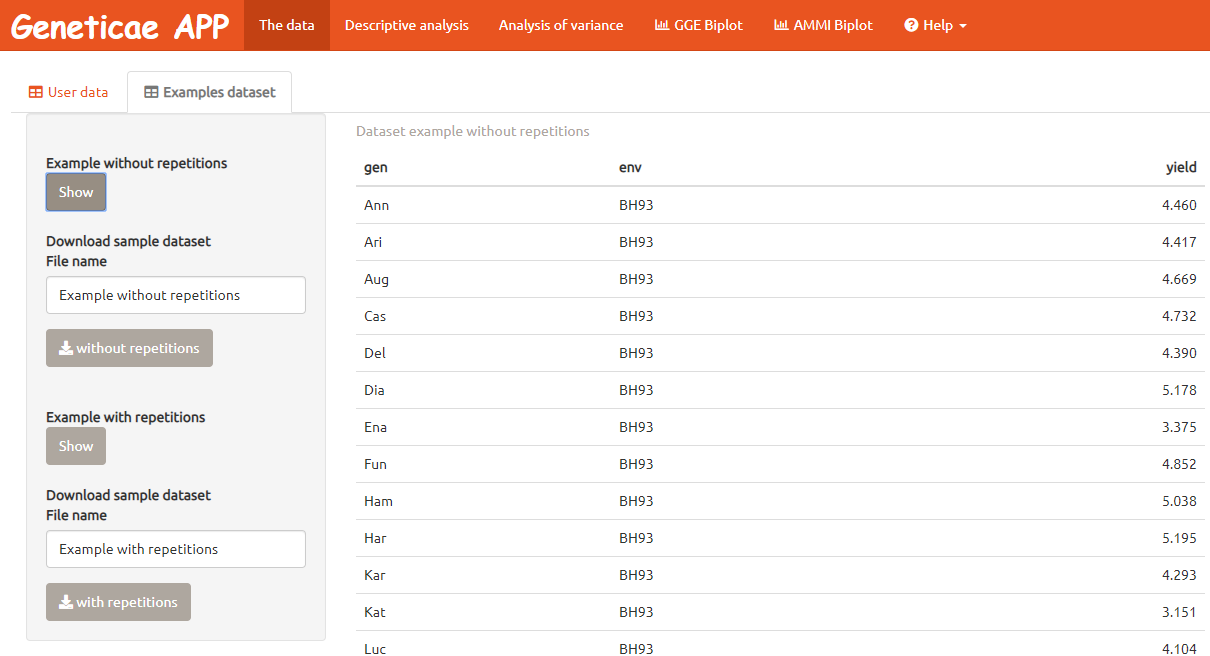
\includegraphics[width=17cm]{./Graficos/Exampledatasets_withrep.png}
	\end{center}
	\caption{Conjunto de datos sin repetición disponible en Shiny Web App}
	\label{fig:fig42}
\end{figure}

\subsection{Análisis descriptivo}

El menú estadística descriptiva le permite describir un conjunto de datos utilizando diagrama de caja (o \emph{boxplot}), gráfico y matriz de correlación y gráfico de interacción.

\subsubsection{\emph{Boxplot}}
El \emph{boxplot} proporciona una medida central, la mediana y una idea de la dispersión a través del rango y el rango intercuartil. La posición de la mediana dentro de la caja y la similitud en la longitud de los bigotes nos dan una idea de la simetría de la distribución. 

Un boxplot intetactivo que compara el caracter cuantitativo de interés a través de genotipos, así como a través de los ambientes se pueden obtener (Figura \ref{fig:fig43},\ref{fig:fig44}).  Estos gráficos se pueden descagar en formato interactivo (.HTML) a partir del boton \emph{Download} (Figura \ref{fig:fig43}), así como también en formato .png (Figura \ref{fig:fig44}).

\begin{figure}[H]
	\begin{center}
		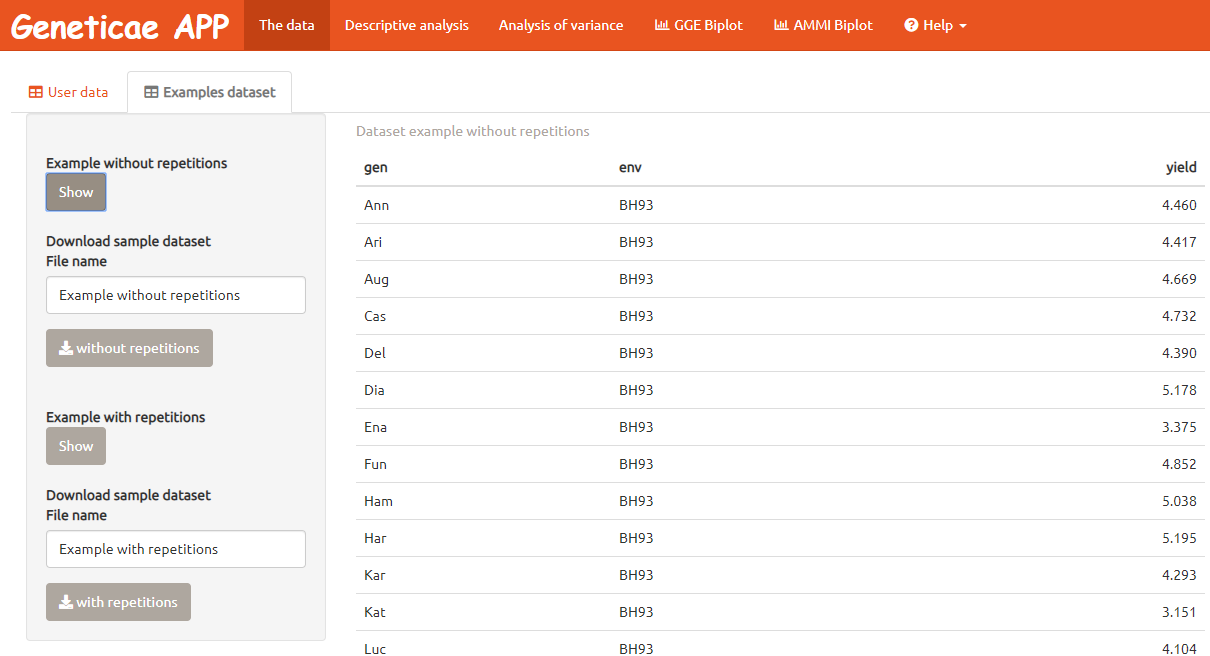
\includegraphics[width=17cm]{./Graficos/Exampledatasets_withrep.png}
	\end{center}
	\caption{Boxplot de genotipos a través de los ambientes para el conjunto de datos Plrv}
	\label{fig:fig43}
\end{figure}


\begin{figure}[H]
	\begin{center}
		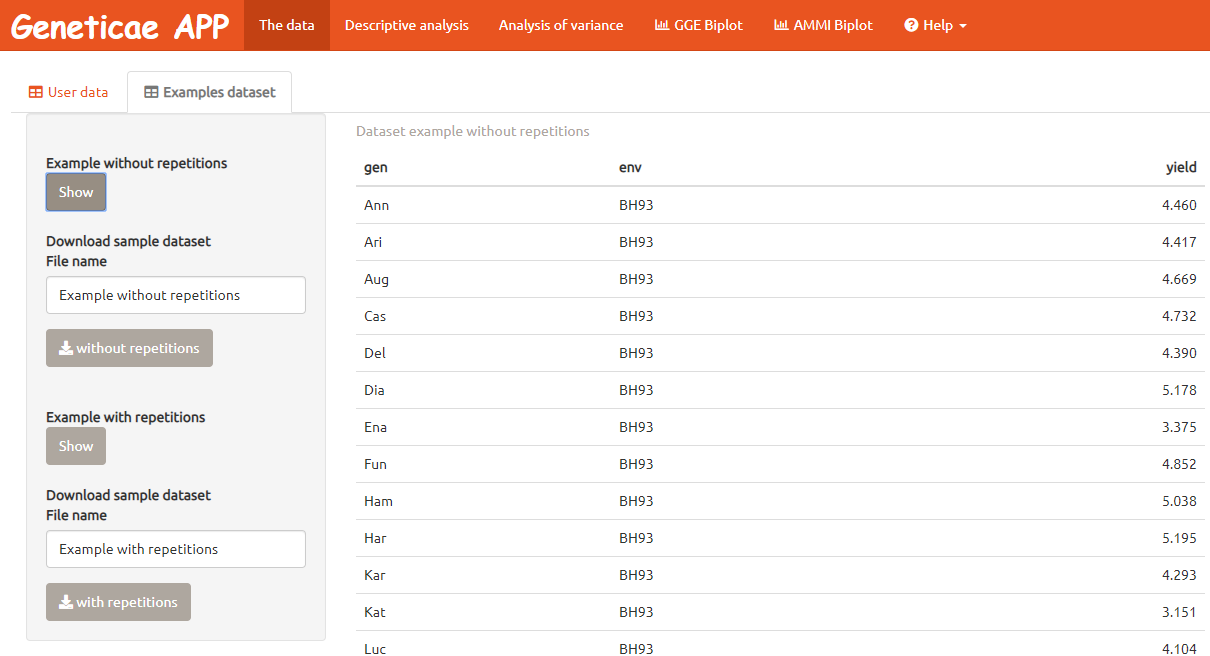
\includegraphics[width=17cm]{./Graficos/Exampledatasets_withrep.png}
	\end{center}
	\caption{Boxplot de ambientes a través de los genotipos para el conjunto de datos Plrv}
	\label{fig:fig44}
\end{figure}

\subsubsection{Gráfico de correlación}
El correlograma o gráfico de correlación muestra la correlación entre pares de variables. Se pueden mostrar las correlaciones de Pearson y Spearman. Las correlaciones positivas se muestran en azul y las negativas en rojo. La intensidad del color y el tamaño del círculo son proporcionales a los coeficientes de correlación. Se pueden trazar ambas correlaciones entre entornos y entre genotipos (Figura \ref{fig:fig45},\ref{fig:fig46}).


\begin{figure}[H]
	\begin{center}
		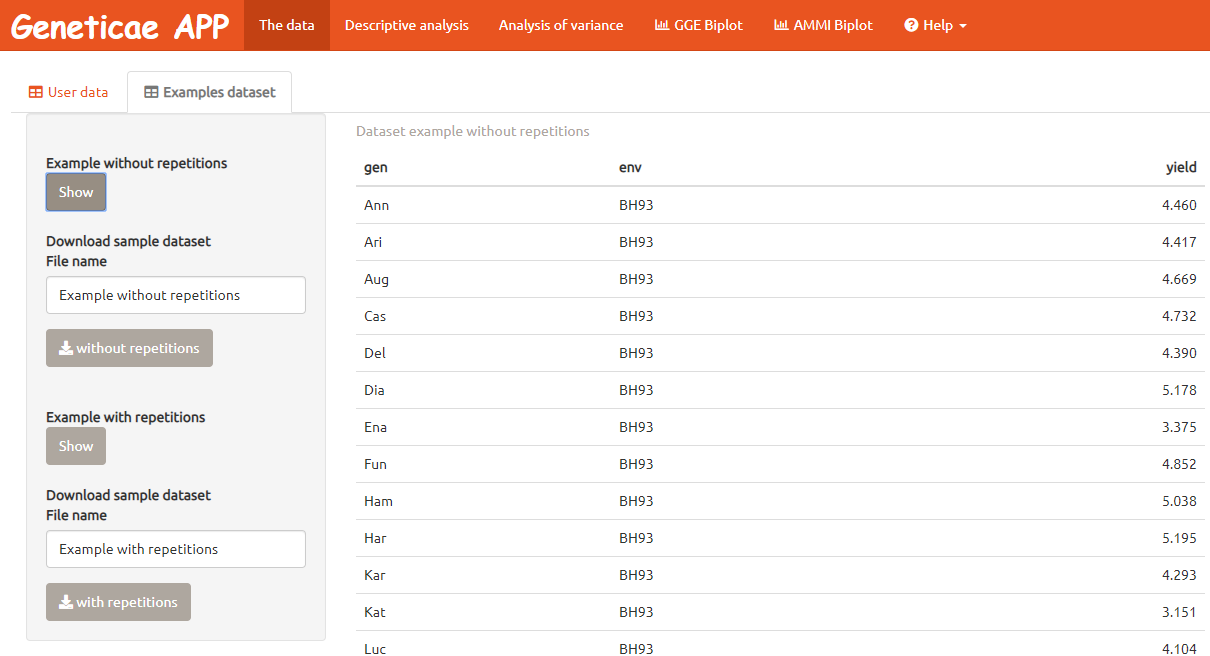
\includegraphics[width=17cm]{./Graficos/Exampledatasets_withrep.png}
	\end{center}
	\caption{Boxplot de genotipos a través de los ambientes para el conjunto de datos Plrv}
	\label{fig:fig45}
\end{figure}


\begin{figure}[H]
	\begin{center}
		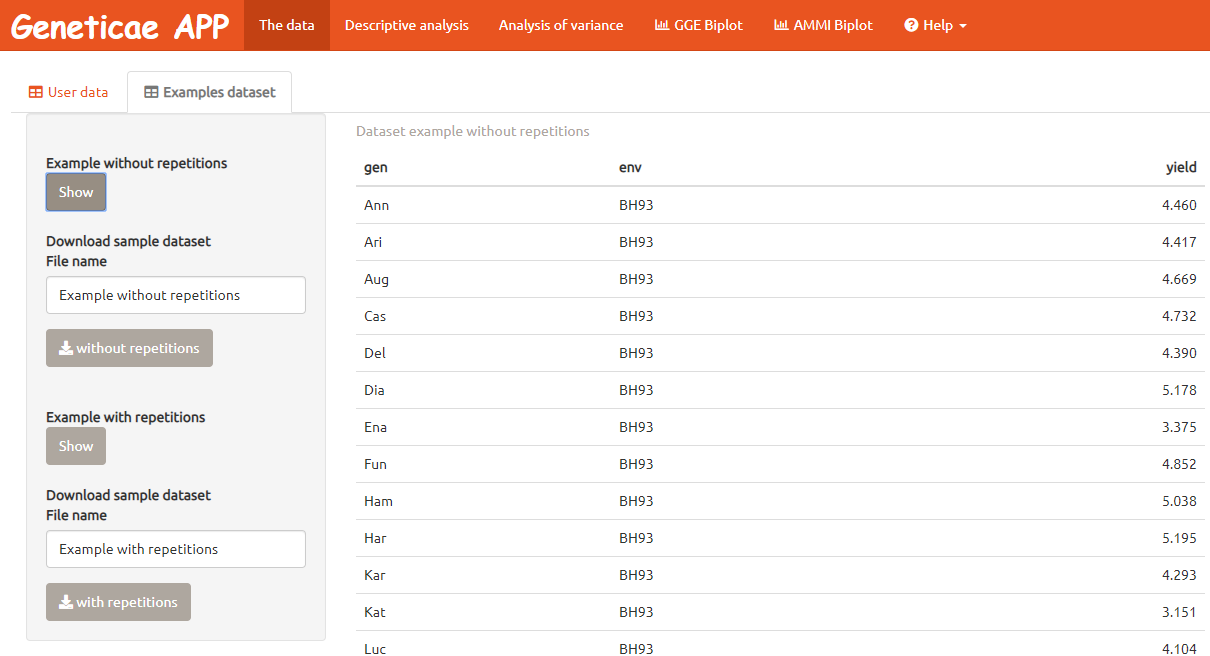
\includegraphics[width=17cm]{./Graficos/Exampledatasets_withrep.png}
	\end{center}
	\caption{Boxplot de ambientes a través de los genotipos para el conjunto de datos Plrv}
	\label{fig:fig46}
\end{figure}

\subsubsection{Matriz de correlación}
Una matriz de correlación se utiliza como una forma de resumir datos. Muestra los coeficientes de correlación de pares de variables. Las correlaciones de Spearman o Pearson se pueden calcular tanto para entornos como para genotipos (Figura \ref{fig:fig47},\ref{fig:fig48}).


\begin{figure}[H]
	\begin{center}
		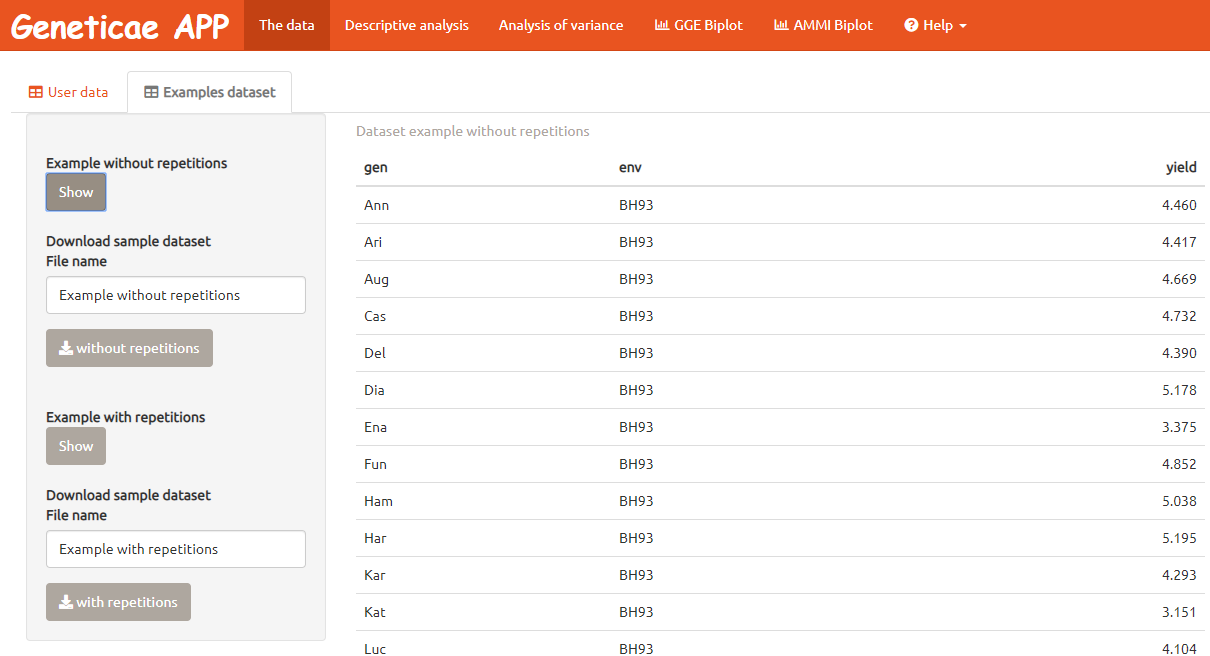
\includegraphics[width=17cm]{./Graficos/Exampledatasets_withrep.png}
	\end{center}
	\caption{Boxplot de genotipos a través de los ambientes para el conjunto de datos Plrv}
	\label{fig:fig47}
\end{figure}


\begin{figure}[H]
	\begin{center}
		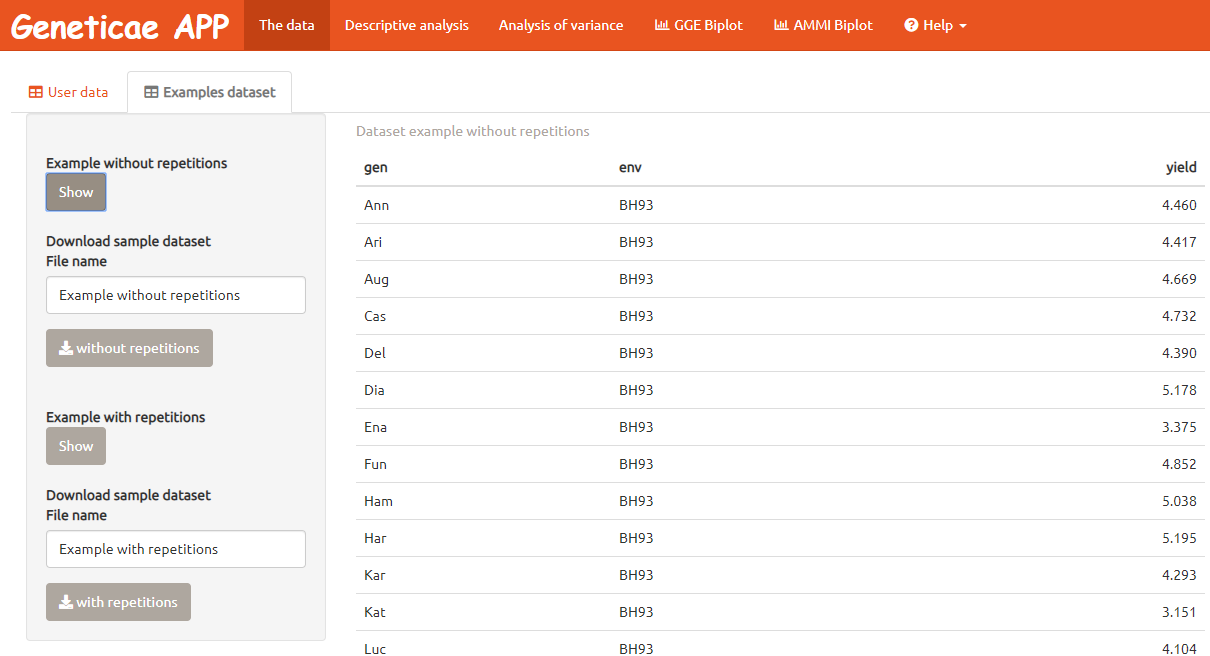
\includegraphics[width=17cm]{./Graficos/Exampledatasets_withrep.png}
	\end{center}
	\caption{Boxplot de ambientes a través de los genotipos para el conjunto de datos Plrv}
	\label{fig:fig48}
\end{figure}

\subsubsection{Gráfico de interacción}
Un diagrama de interacción es una representación visual de la interacción entre los efectos de dos factores, o entre un factor y una variable numérica. 

Se puede obtener el gráfico interactivo que muestra el cambio en el efecto genotípico a través de los entornos y también el que muestra el cambio en el efecto ambiental a través de los genotipos (Figura \ref{fig:fig49},\ref{fig:fig410}). Es posible descargarlo en formato interactivo (.HTML) a partir del boton \emph{Download} (Figura \ref{fig:fig49}), así como también en formato .png como se muestra en la Figura \ref{fig:fig410}.


\begin{figure}[H]
	\begin{center}
		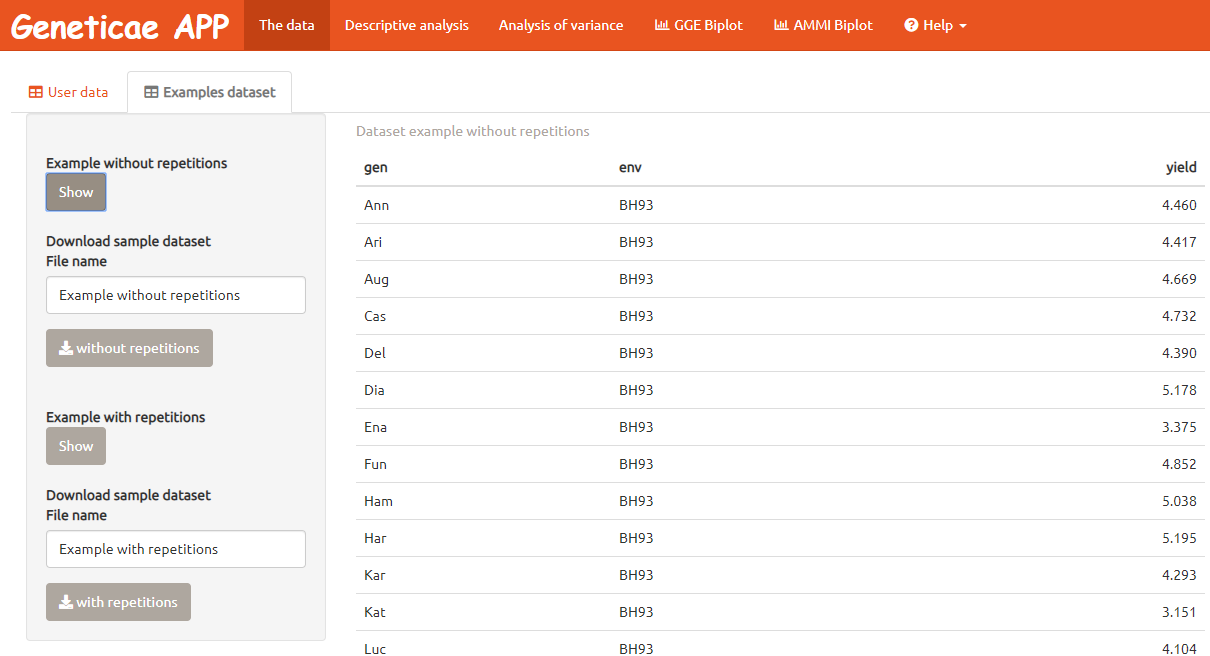
\includegraphics[width=17cm]{./Graficos/Exampledatasets_withrep.png}
	\end{center}
	\caption{Boxplot de genotipos a través de los ambientes para el conjunto de datos Plrv}
	\label{fig:fig49}
\end{figure}


\begin{figure}[H]
	\begin{center}
		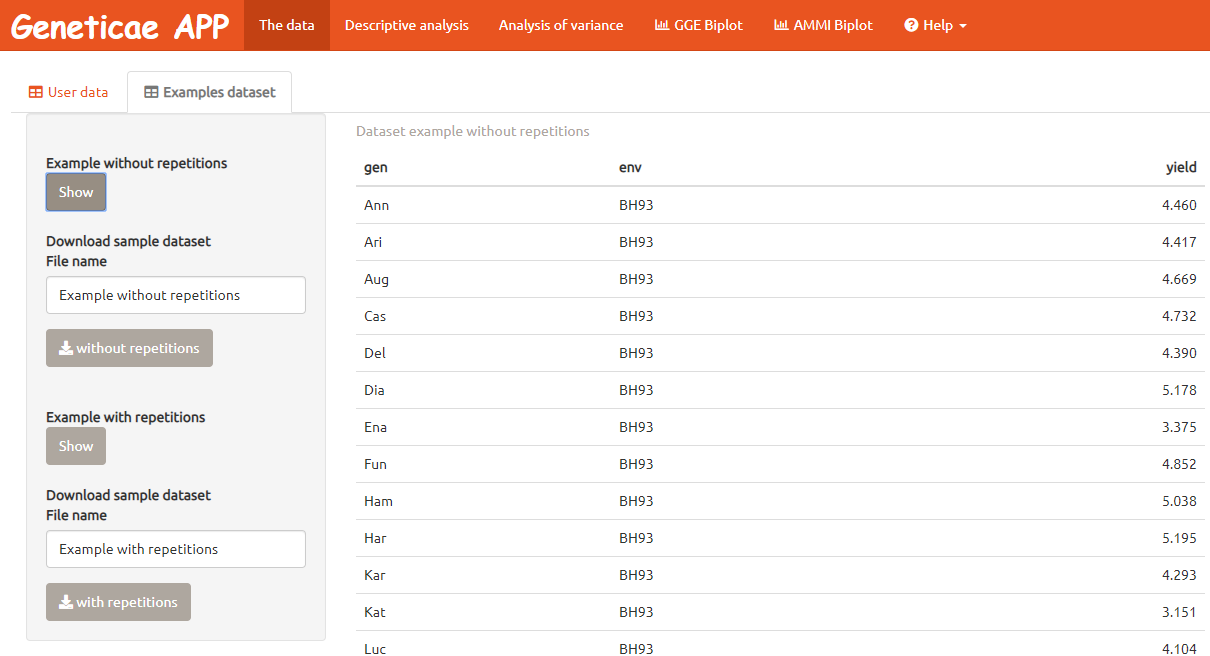
\includegraphics[width=17cm]{./Graficos/Exampledatasets_withrep.png}
	\end{center}
	\caption{Boxplot de ambientes a través de los genotipos para el conjunto de datos Plrv}
	\label{fig:fig410}
\end{figure}


\subsection{Análisis de la variancia}


\subsection{Biplot GGE}
El biplot GGE aborda visualmente muchos problemas relacionados con la evaluación de los genotipo y ambientes de prueba. En el caso de repeticiones disponibles en el conjunto de datos, se obtiene el valor fenotípico promedio para cada combinación de genotipo y ambiente. Los valores faltantes no están permitidos.


\subsection{Biplot GE}

\subsection{Ayuda}
%\include{capitulo3}
\chapter{Conclusión}

Como resultados del presente trabajo fue posible:\\

\textbf{Mostrar un flujo de trabajo reproducible para la construcción de paquetes de R}. El mismo se puede utilizar de ejemplo para el desarrollo de nuevos paquetes o imitar la construcción del paquete \emph{geneticae} objeto de este trabajo. \\

\textbf{Construir un paquete de R llamado \emph{geneticae}} para el análisis de datos provenientes de EMA. El mismo es de gran utilidad ya que incluye metodología recientemente publicada además de la reunir las herramientas más utilizadas por los fitomejoradores para el análisis gráfico. En el momento de la escritura de este informe, pasaron 3 semanas desde su publicación en el repositorio CRAN y cuenta con más de 400 descargas, a pesar de que aún no se ha hecho difusión del paquete. \\

\textbf{Desarrollar una aplicación web Shiny denominada \emph{Geneticae}}, la cual es de suma importancia para aquellos analistas no familiarizados con la programación. Esta es de libre acceso mediante conexión a internet que permite realizar los principales análisis implementados en el paquete sin necesidad de escribir líneas de código. \\

Se plantea como línea futura, continuar con la inclusión de los avances metodologicos que se vayan publicando en el contexto de datos provenientes de EMA tanto en el paquete como en la aplicación web Shiny. 









\appendix
%% Cap'itulos incluidos despues del comando \appendix aparecen como ap'endices
%% de la tesis.
%% Los cap'itulos inician con \chapter{T'itulo}, estos aparecen numerados y
%% se incluyen en el 'indice general.
%%
%% Recuerda que aqu'i ya puedes escribir acentos como: 'a, 'e, 'i, etc.
%% La letra n con tilde es: 'n.


%\setcounter{section}{1}
\chapter{Hoja de referencia Shiny}
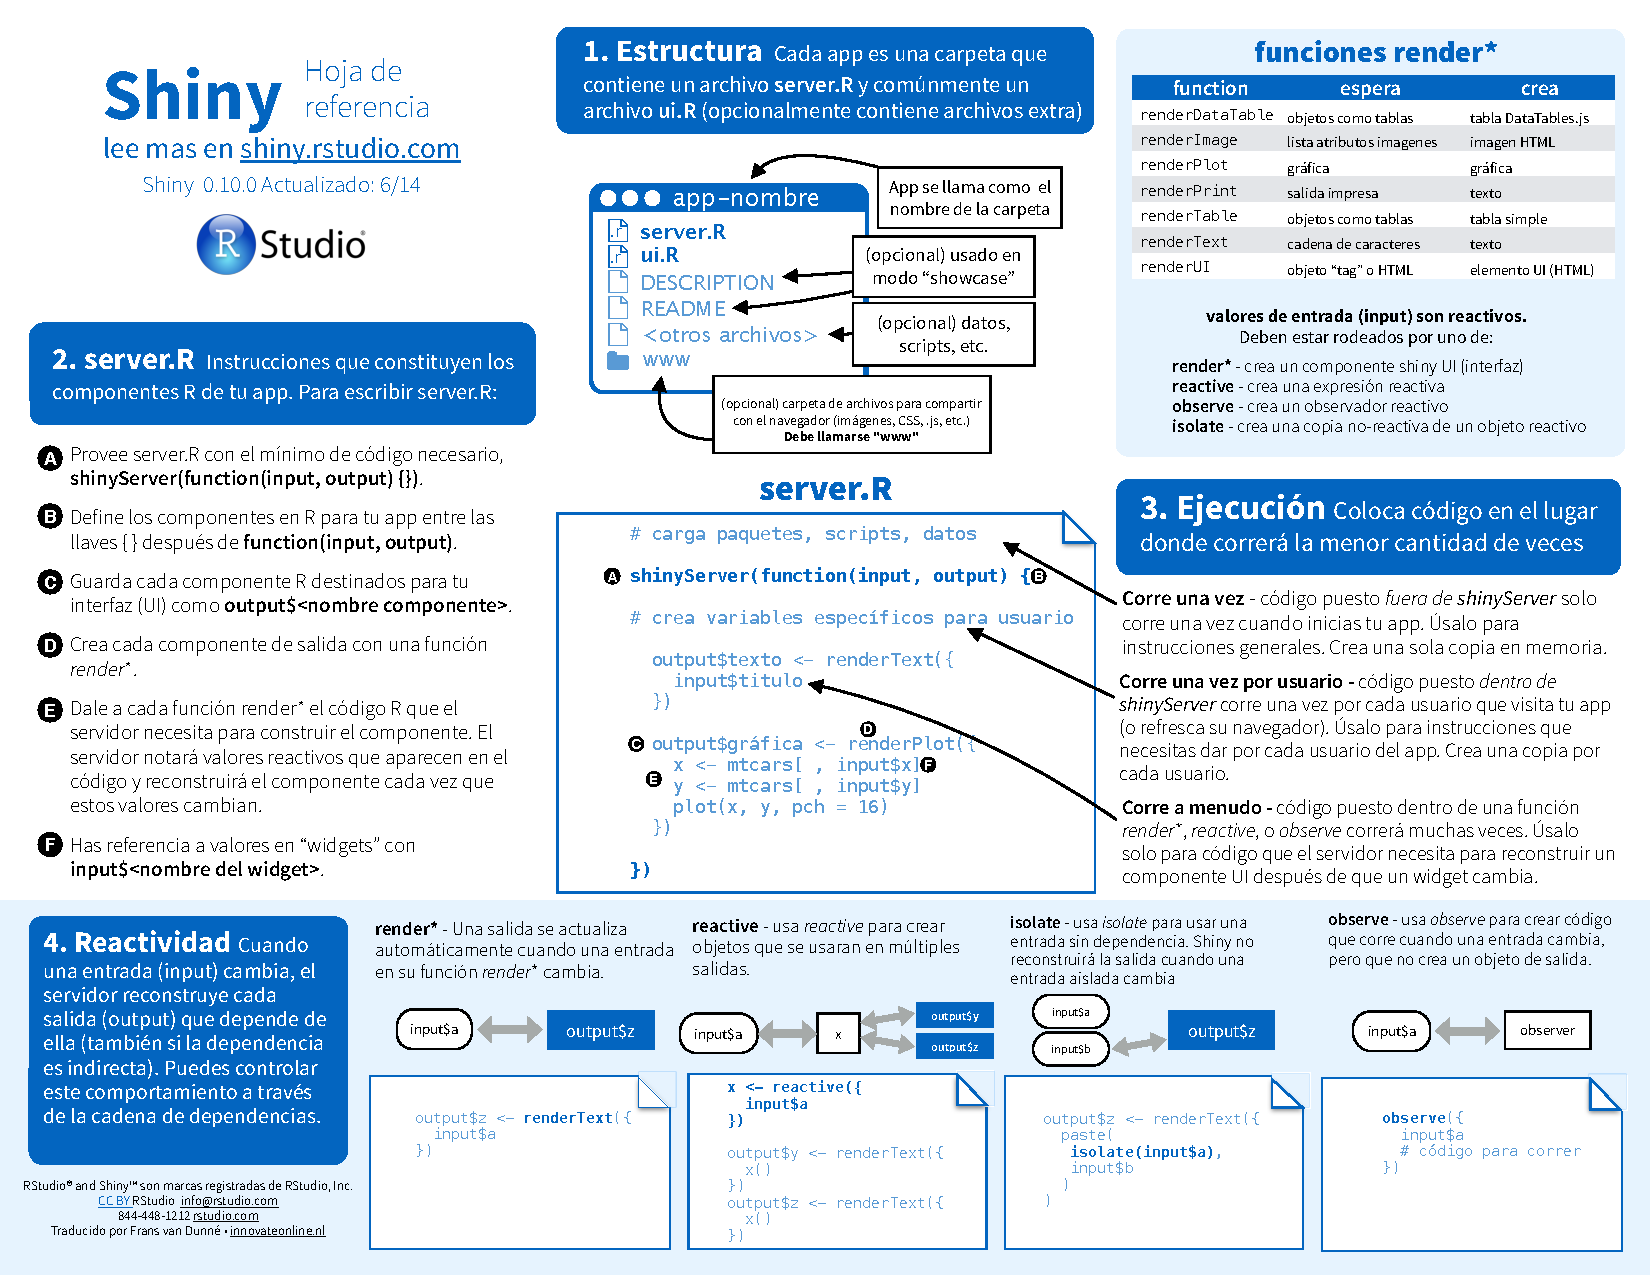
\includepdf[pages={1-2},scale=.78,pagecommand={},angle=90]{shiny-spanish.pdf}

%% Los cap'itulos inician con \chapter{T'itulo}, estos aparecen numerados y
%% se incluyen en el 'indice general.
%%
%% Recuerda que aqu'i ya puedes escribir acentos como: 'a, 'e, 'i, etc.
%% La letra n con tilde es: 'n.


%\setcounter{section}{1}
\chapter{Guías para usuario de Geneticae APP}


%% Los cap'itulos inician con \chapter{T'itulo}, estos aparecen numerados y
%% se incluyen en el 'indice general.
%%
%% Recuerda que aqu'i ya puedes escribir acentos como: 'a, 'e, 'i, etc.
%% La letra n con tilde es: 'n.


%\setcounter{section}{1}
\chapter{Código R de Geneticae APP}



%% Incluir la bibliograf'ia. Mirar el archivo "biblio.bib" para m'as detales
%% y un ejemplo.

\bibliography{biblio}

\end{document}
